\section{问题二：视觉刺激到头皮脑电的正向计算模型}

\subsection{问题重述与分析}

题目要求说明视觉刺激经 LGN 和皮层后如何形成头皮脑电，解释左、右三角提示可能产生差异的计算机制，并提出可用于区分两类提示响应的特征表示\cite{problem2026}。该问的主要困难有三点：左右图形互为镜像，若把空间图过早压成全局均值就会丢失差异来源；五个内部源代理只对应三个电极，不能从观测端唯一反演源；条件差异既要由模型产生，也要经真实脑电的留出记录检验。

本文沿正向方向建立计算链，并对三类结果分别评价：检查镜像图像是否经空间化前端形成模型内部差异；以整份记录留出检验模拟 ERP 对真实 ERP 的波形解释能力；直接从真实单试次脑电构造固定维度特征并检验跨记录分类。模型内部可分性不能替代真实传感器上的泛化证据。

\subsection{模型假设与符号说明}

\subsubsection{模型假设}

\begin{enumerate}
\def\labelenumi{\arabic{enumi}.}
\tightlist
\item 输入图像矩阵及共同背景矩阵代表模型使用的视觉亮度结构；左右提示的相对差分保留明暗符号与空间位置。
\item VisCue 对齐的提示起点取 0 ms，提示显示区间按实现设置为 \([0,200)\) ms。提示消失后，LGN 和皮层状态按方程自然衰减。
\item 三组兴奋-抑制活动和五个源均作为低维功能代理；它们刻画模型计算路径，不赋予具体解剖脑区含义。
\item 电极和乳突参考使用规范头坐标及固定点偶极近似。源坐标、方向和导电率采用统一设定，不从留出记录重新估计。
\item 外层验证单位为 MAT 记录。四份文件没有可核实的受试者身份，因此结果只称记录留出验证。
\item 问题二主模型模拟提示输入，不在约 2.2 s 加入目标刺激。模型输出与真实完整试次的晚期信号比较时，保留该事件上下文差异作为解释限制。
\end{enumerate}

\textbf{表 1 主要符号说明}

\begin{longtable}[]{@{}lll@{}}
\toprule
符号 & 含义 & 单位或维度 \\
\midrule
\endhead
\(X_s(x,y)\) & 相对共同背景的带符号提示图像，\(s\in\{L,R\}\) & 归一化亮度差 \\
\(D,A,T\) & 中心—周围响应、适应状态与适应后瞬态 & 相对输入量 \\
\(U_{\rm ON},U_{\rm OFF}\) & ON、OFF 分支的中继输入 & 相对特征量 \\
\(R,N,Q\) & TCR、IN、TRN 三类神经群的相对活动 & \([0,1]\) \\
\(\Phi_{\beta,\theta}\) & 截断逻辑激活函数 & \([0,1]\) \\
\(B,H_L,H_R\) & 早期方向能量与左右三角构型图 & 相对特征量 \\
\(d_L,d_R\) & 左右模板偏好驱动 & 相对特征量 \\
\(E_{p,c},I_{p,c}\) & 第 \(p\) 组、第 \(c\) 通道的兴奋和抑制活动 & \([0,1]\) \\
\(h_\tau\) & 因果突触响应核 & --- \\
\(P_{p,c}\) & 群体状态经突触核滤波后的源代理分量 & 相对活动量 \\
\(\mathbf q(t)\) & 五维功能源代理 & 相对活动量 \\
\(G\) & 源代理到 F3、Fz、F4 的固定正向映射 & \(3\times5\) \\
\(L_{ej},G_{ej}\) & 点偶极近似下的导联场系数与参考电极修正 & --- \\
\(\tau_s,g_i,\tau_a\) & 皮层时间常数、抑制增益、LGN 适应时间常数 & ms、无量纲、ms \\
\(\alpha\) & 每折由训练 ERP 估计的共享有符号幅度因子 & 相对尺度 \\
\(u_0,u_1,u_2\) & 共同、侧化、形状三个正交观测模式 & --- \\
\(\mathbf z\) & 单试次九维 ERP 特征向量 & \(\mathbb R^9\) \\
\bottomrule
\end{longtable}

\subsection{数据与视觉刺激编码}

实测脑电取自第一问清洗后的四份 MAT 记录，按通道标签重排为 F3、Fz、F4，采样率为 \(128\) Hz。每个提示试次先减去提示前 \([-200,0)\) ms 均值，再计算条件平均 ERP。可用于左右提示分析的试次如表 2 所示。

\textbf{表 2 Stage1 左右提示试次数}

\begin{longtable}[]{@{}llll@{}}
\toprule
记录 & 实验任务 & 左提示 & 右提示 \\
\midrule
\endhead
A-1 & Task1 & 29 & 25 \\
A-2 & Task1 & 45 & 35 \\
B-1 & Task2 & 41 & 42 \\
B-2 & Task2 & 37 & 43 \\
合计 & & 152 & 145 \\
\bottomrule
\end{longtable}

四份记录合计 297 个提示试次，左提示 152 次、右提示 145 次。单条记录有 103 个可用时间点，覆盖 0 至 \(796.875\) ms；\(128\) Hz 网格不含恰好 \(800\) ms 的采样点。

图~\ref{fig:q2_measured_erp} 展示第一问清洗数据中四份记录的 F3、Fz、F4 左右提示条件平均 ERP。每行对应一份记录，阴影为均值的近似 95\% 置信带。该图用于描述实测输入的记录内波形和变异范围；条件均值的分离不等同于单试次分类能力，也不作为模型参数拟合的额外目标。

\begin{figure}[H]
\centering
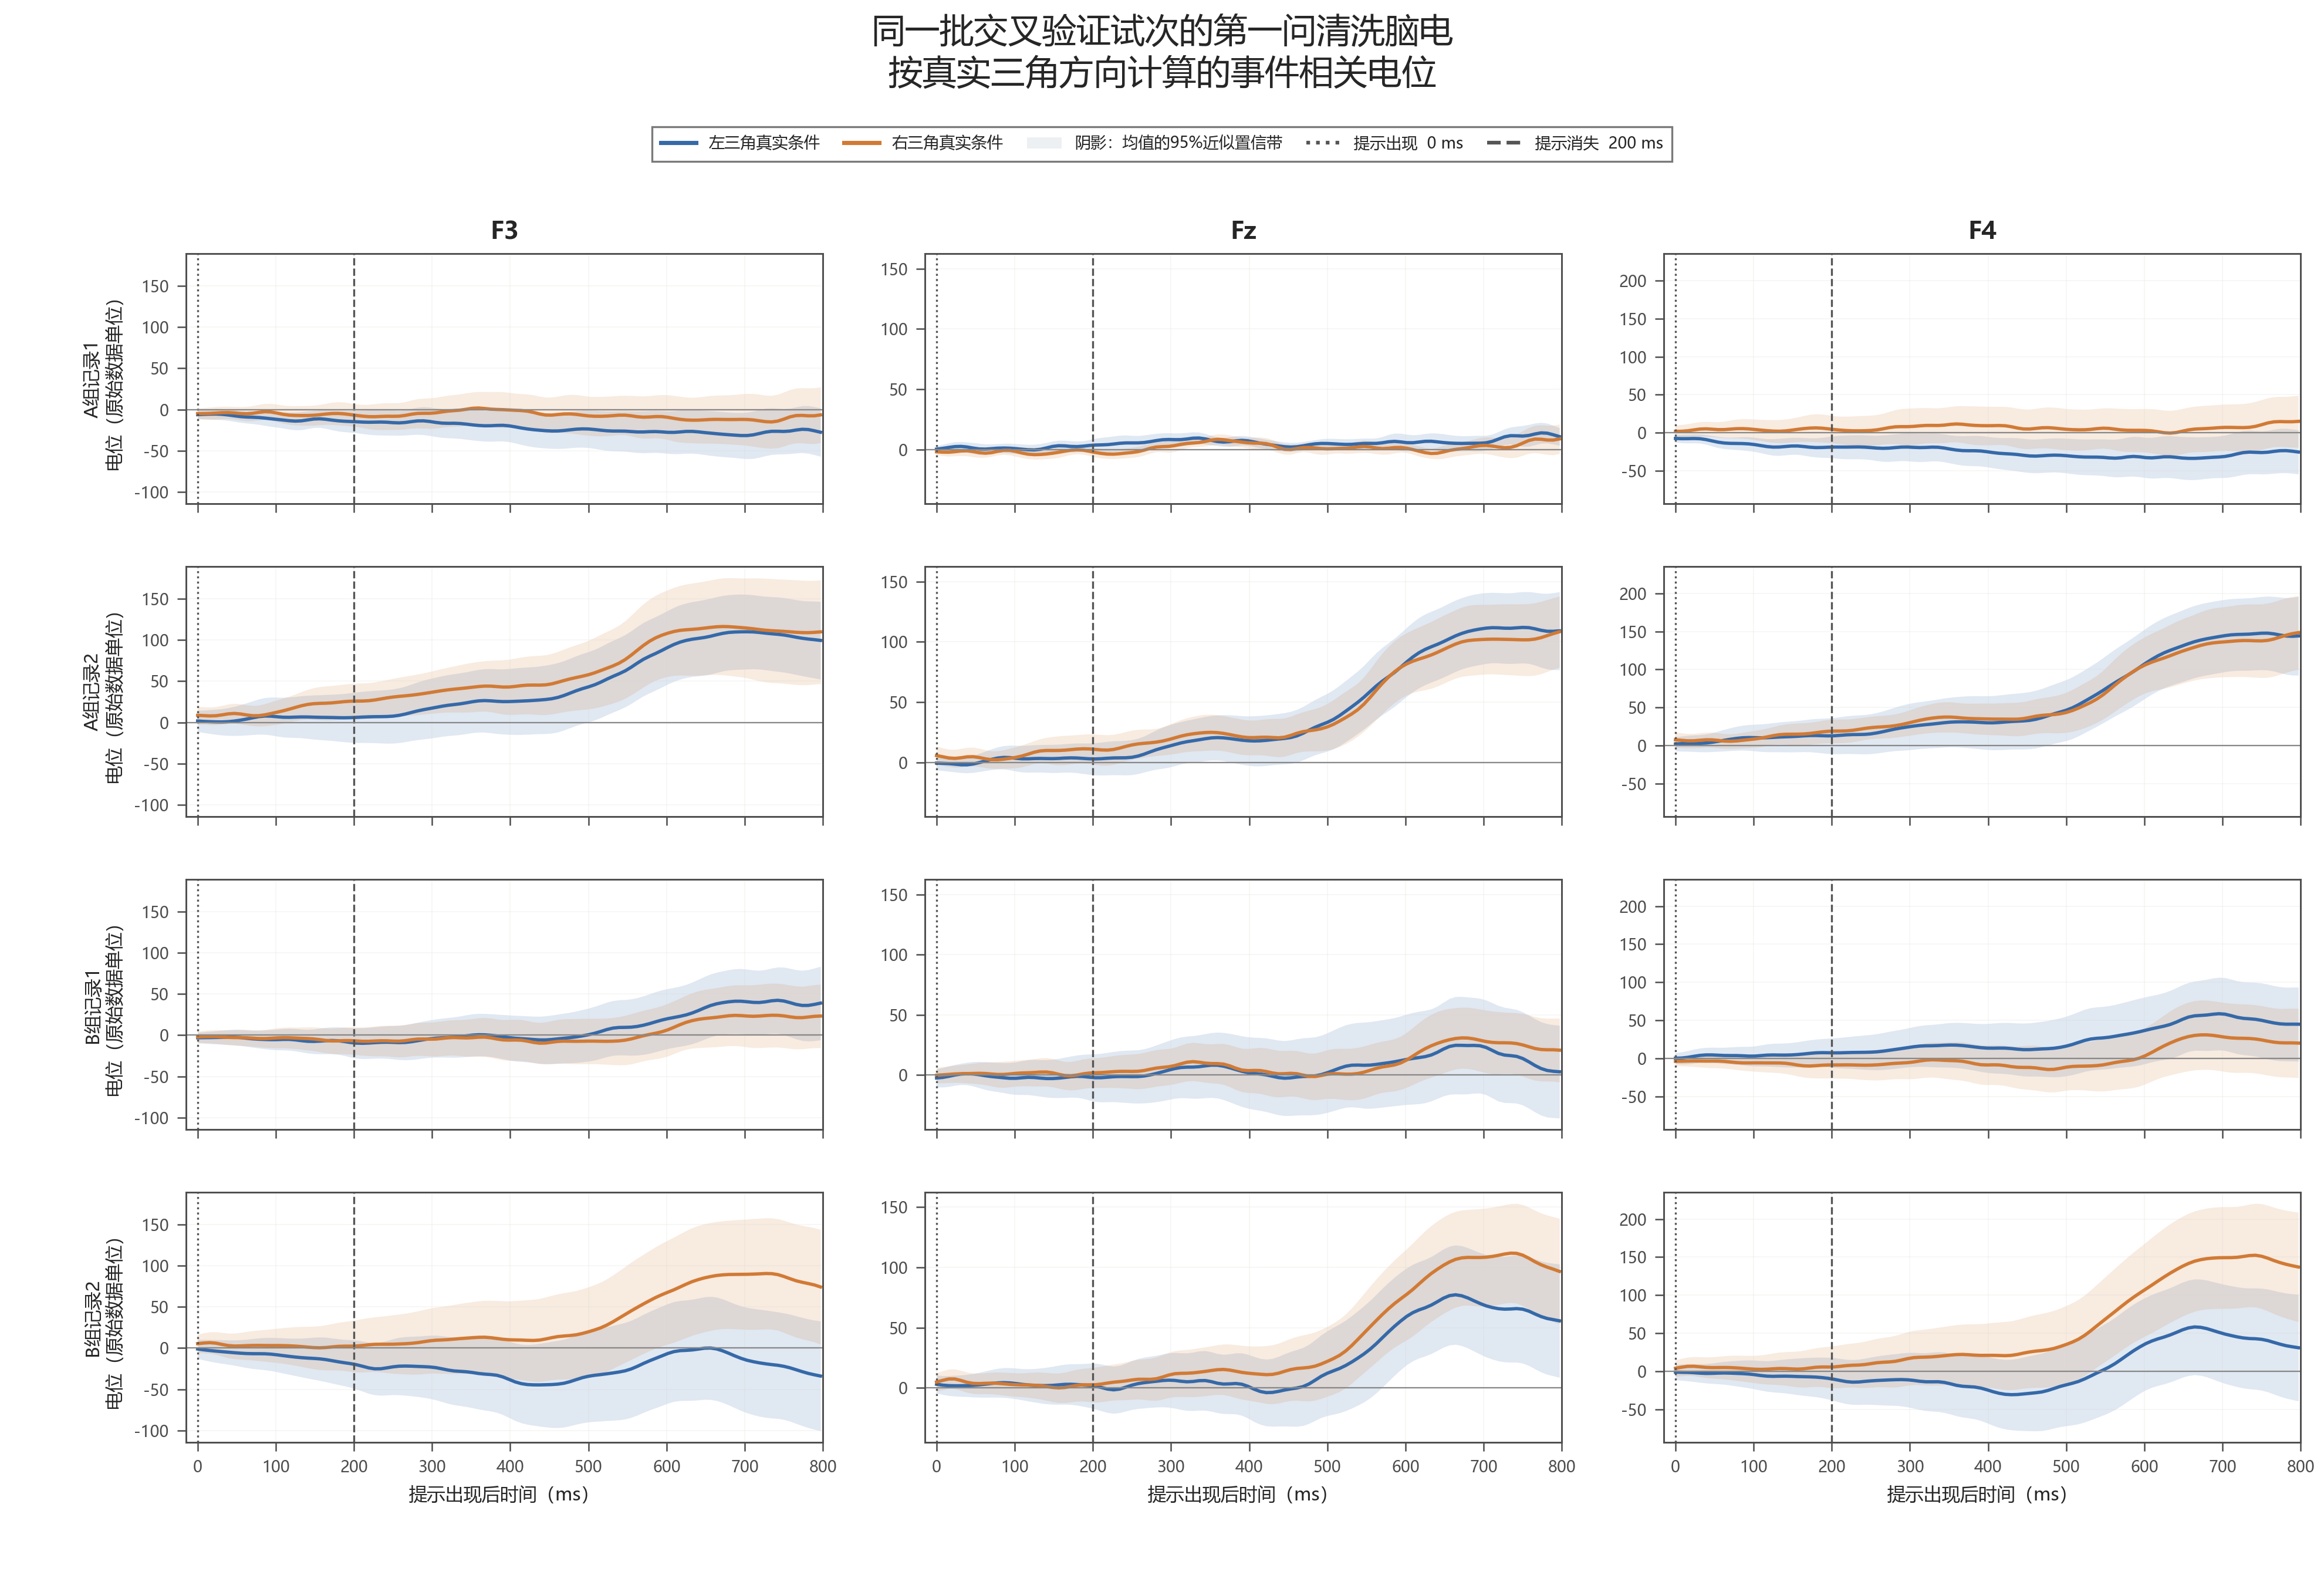
\includegraphics[width=0.96\textwidth]{src/C/q2/output/final_pic/03_同批试次_真实脑电左右响应.png}
\caption{四份记录中左右提示条件的实测 ERP。实线为按提示方向分组的均值，阴影为均值的近似 95\% 置信带；纵轴沿用第一问清洗数据的原始数据单位。}\label{fig:q2_measured_erp}
\end{figure}

模型将 \(256\times256\) 灰度提示图与共同圆形背景图相减并按 255 归一化：

\begin{equation}
X_s(x,y)=\frac{I_s(x,y)-B(x,y)}{255},\qquad s\in\{L,R\}.
\end{equation}

共同圆环在差分中抵消，三角形相对背景的像素对比约为 \(-0.451\)；左右差分图为严格水平镜像。模型以 0 ms 提示出现和 200 ms 提示消失构造外部驱动，后续活动由模型状态递推得到。

图~\ref{fig:q2_stimulus} 展示镜像提示在方向和三角形构型前端中的空间响应。图中热图是模型内部特征，不是实测脑电或源定位结果。

\begin{figure}[H]
\centering
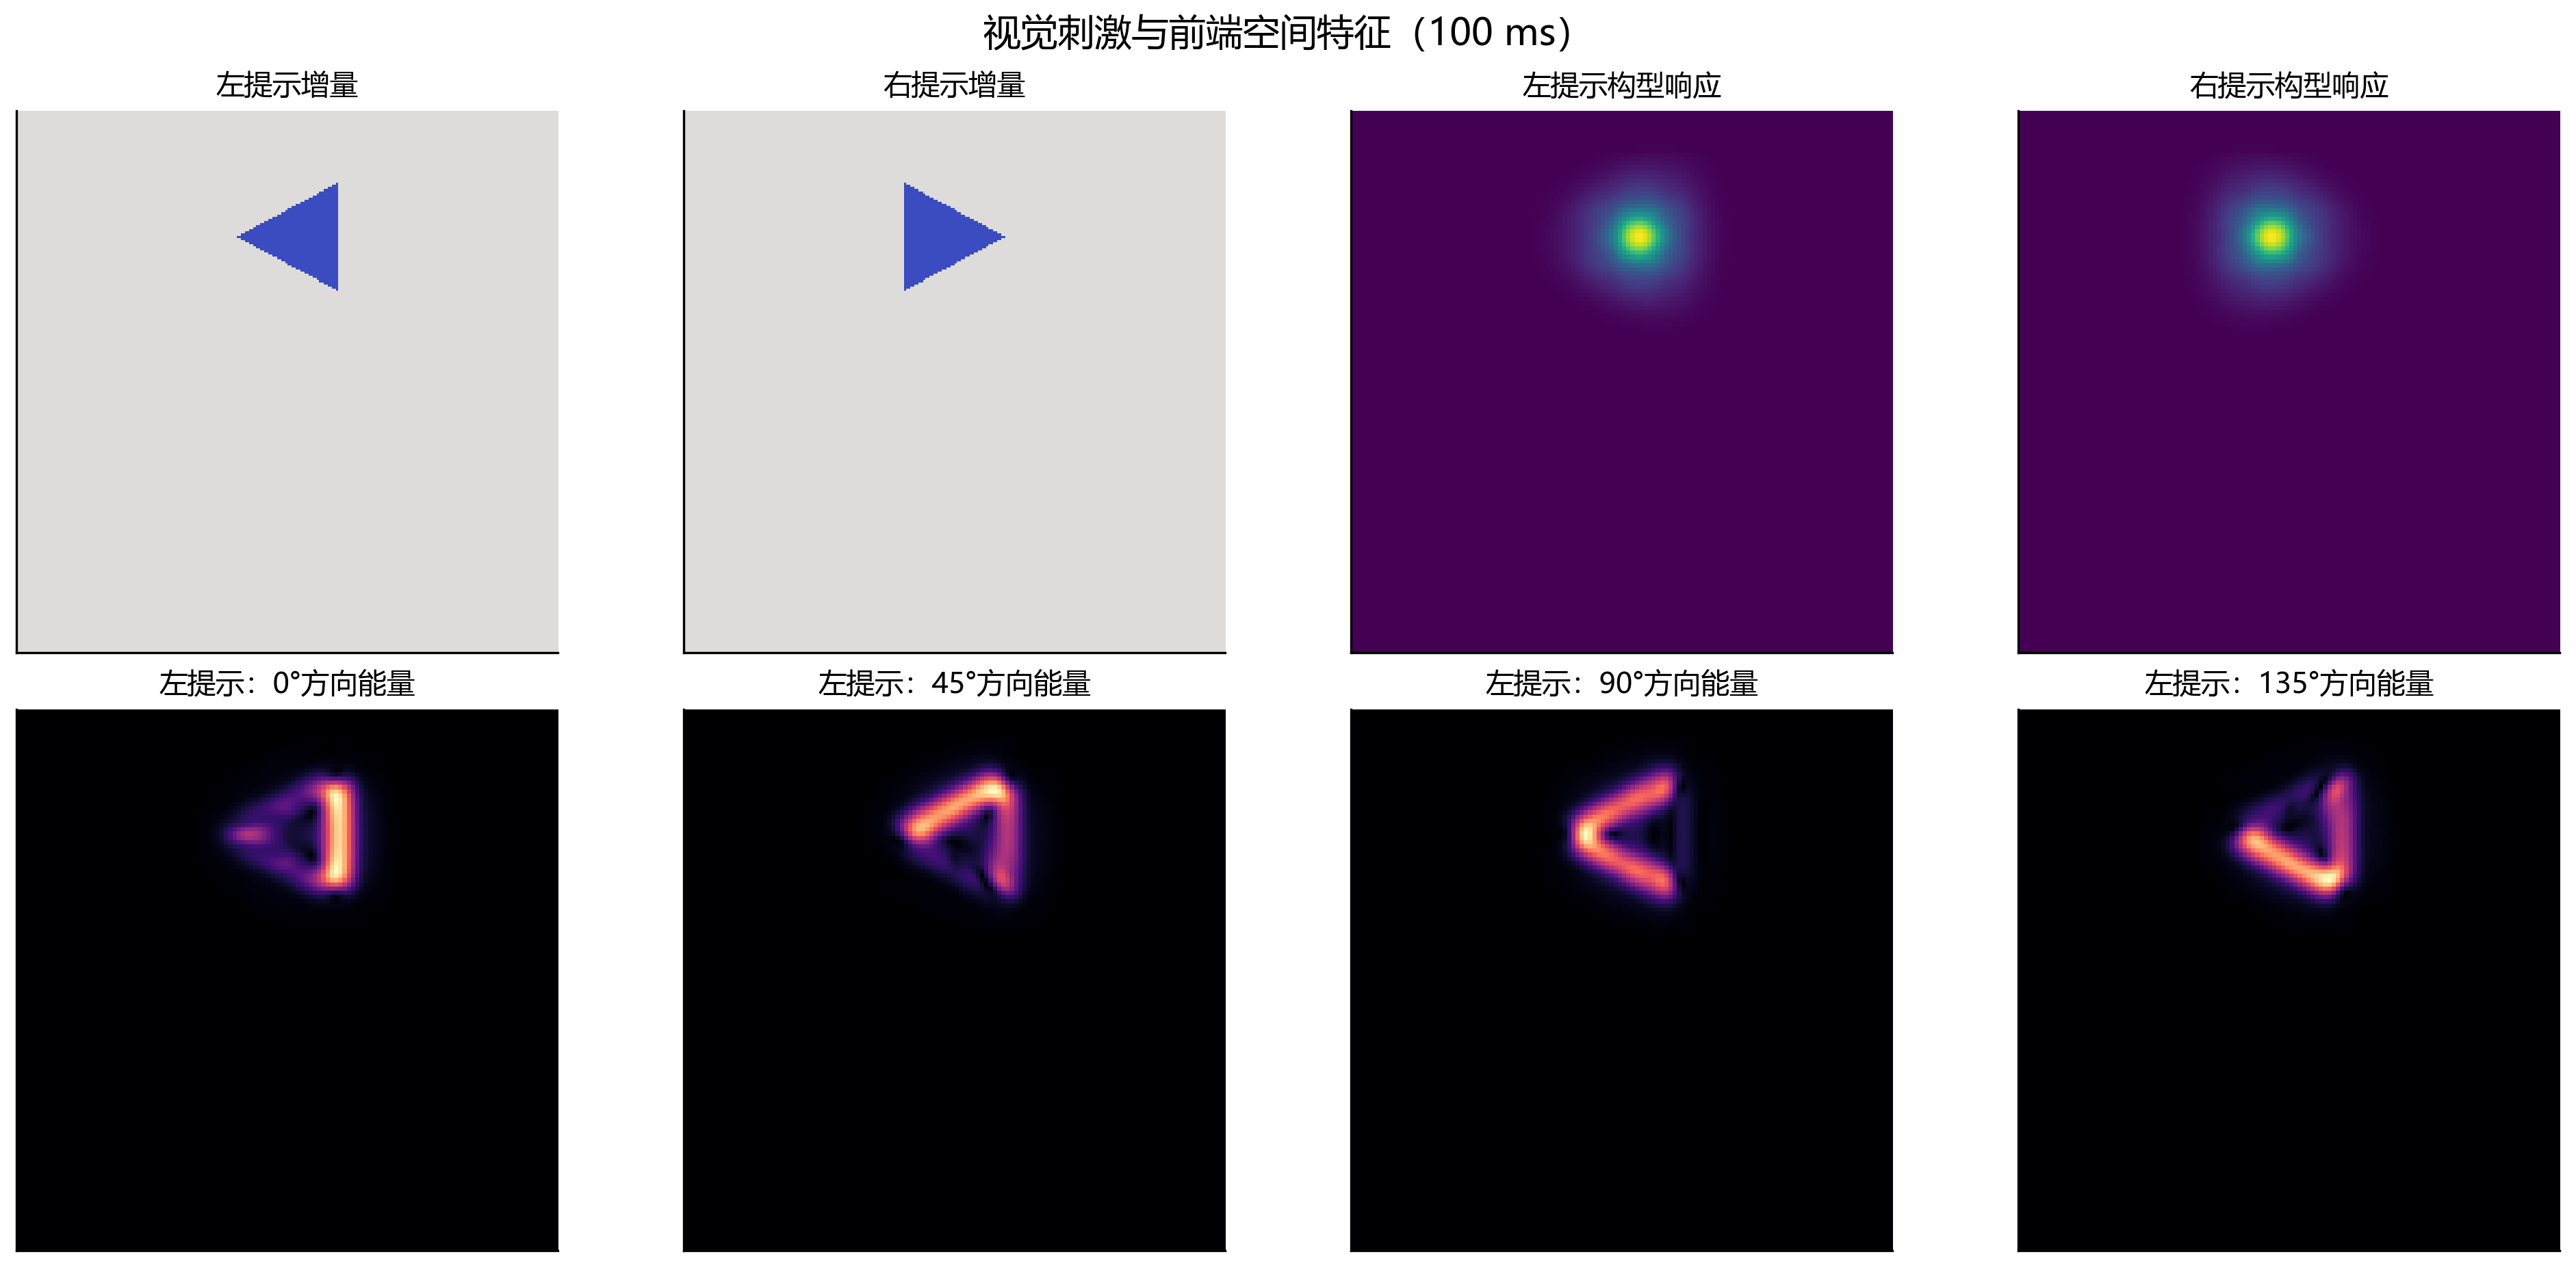
\includegraphics[width=0.96\textwidth]{src/C/q2/documents/figures/视觉刺激与前端空间特征.png}
\caption{左右视觉提示与前端空间特征}\label{fig:q2_stimulus}
\end{figure}

\subsection{正向脑电计算模型}

\subsubsection{LGN ON/OFF 中继}

中心—周围差分用于突出局部亮度边界：

\begin{equation}
D_t=G_{\sigma_c}*X_t-G_{\sigma_s}*X_t,\qquad \sigma_c=1.5\text{ px},\quad \sigma_s=4\text{ px}.
\end{equation}

随后以一阶适应状态区分持续输入与瞬态变化，并将响应拆分为 ON、OFF 两支：

\begin{equation}
A_{t+\Delta t}=A_t+\frac{\Delta t}{\tau_a}(D_t-A_t),\qquad T_t=D_t-A_t,
\end{equation}

\begin{equation}
U_{\rm ON}=0.8[T_t]_++0.2[D_t]_+,\qquad
U_{\rm OFF}=0.8[-T_t]_++0.2[-D_t]_+,
\end{equation}

其中 \([x]_+=\max(x,0)\)。中继细胞 TCR、中间神经元 IN 和网状丘脑核 TRN 构成简化反馈回路，其稳态目标活动和一阶状态更新写为

\begin{equation}
\begin{aligned}
R^*&=\Phi_{4,0.5}(2.2U-0.9N-0.8Q),\\
N^*&=\Phi_{4,0.5}(1.2U+0.7R),\\
Q^*&=\Phi_{4,0.5}(0.9R),\\
R_{t+\Delta t}&=R_t+\frac{\Delta t}{18}(R^*-R_t),\\
N_{t+\Delta t}&=N_t+\frac{\Delta t}{12}(N^*-N_t),\\
Q_{t+\Delta t}&=Q_t+\frac{\Delta t}{25}(Q^*-Q_t).
\end{aligned}
\end{equation}

激活函数采用零点归零、输出限于 \([0,1]\) 的截断逻辑函数：

\begin{equation}
\Phi_{\beta,\theta}(z)=\operatorname{clip}_{[0,1]}\!\left[
\frac{\sigma(\beta(z-\theta))-\sigma(-\beta\theta)}
{1-\sigma(-\beta\theta)}\right],\qquad \sigma(z)=\frac{1}{1+e^{-z}}.
\end{equation}

ON 和 OFF 分支各自递推 \(R,N,Q\)，所有状态初值为 0，积分步长为 1 ms。适应时间常数 \(\tau_a\) 在 40、60、80、100、120、140、160 ms 七个候选值中由训练数据拟合。

图~\ref{fig:q2_lgn_mean} 展示模型的群体平均 ON/OFF 活动：提示出现和 200 ms 提示消失分别形成瞬态驱动，随后状态自然衰减；纵轴为相对活动量。图~\ref{fig:q2_lgn_peaks} 展示 0--800 ms 内各空间通道的 TCR 峰值，左右条件的镜像位置结构可在空间图上比较。两图均为同一组标准刺激经模型计算并按入选试次记录构成加权后的结果，不是实测神经元放电。

\begin{figure}[H]
\centering
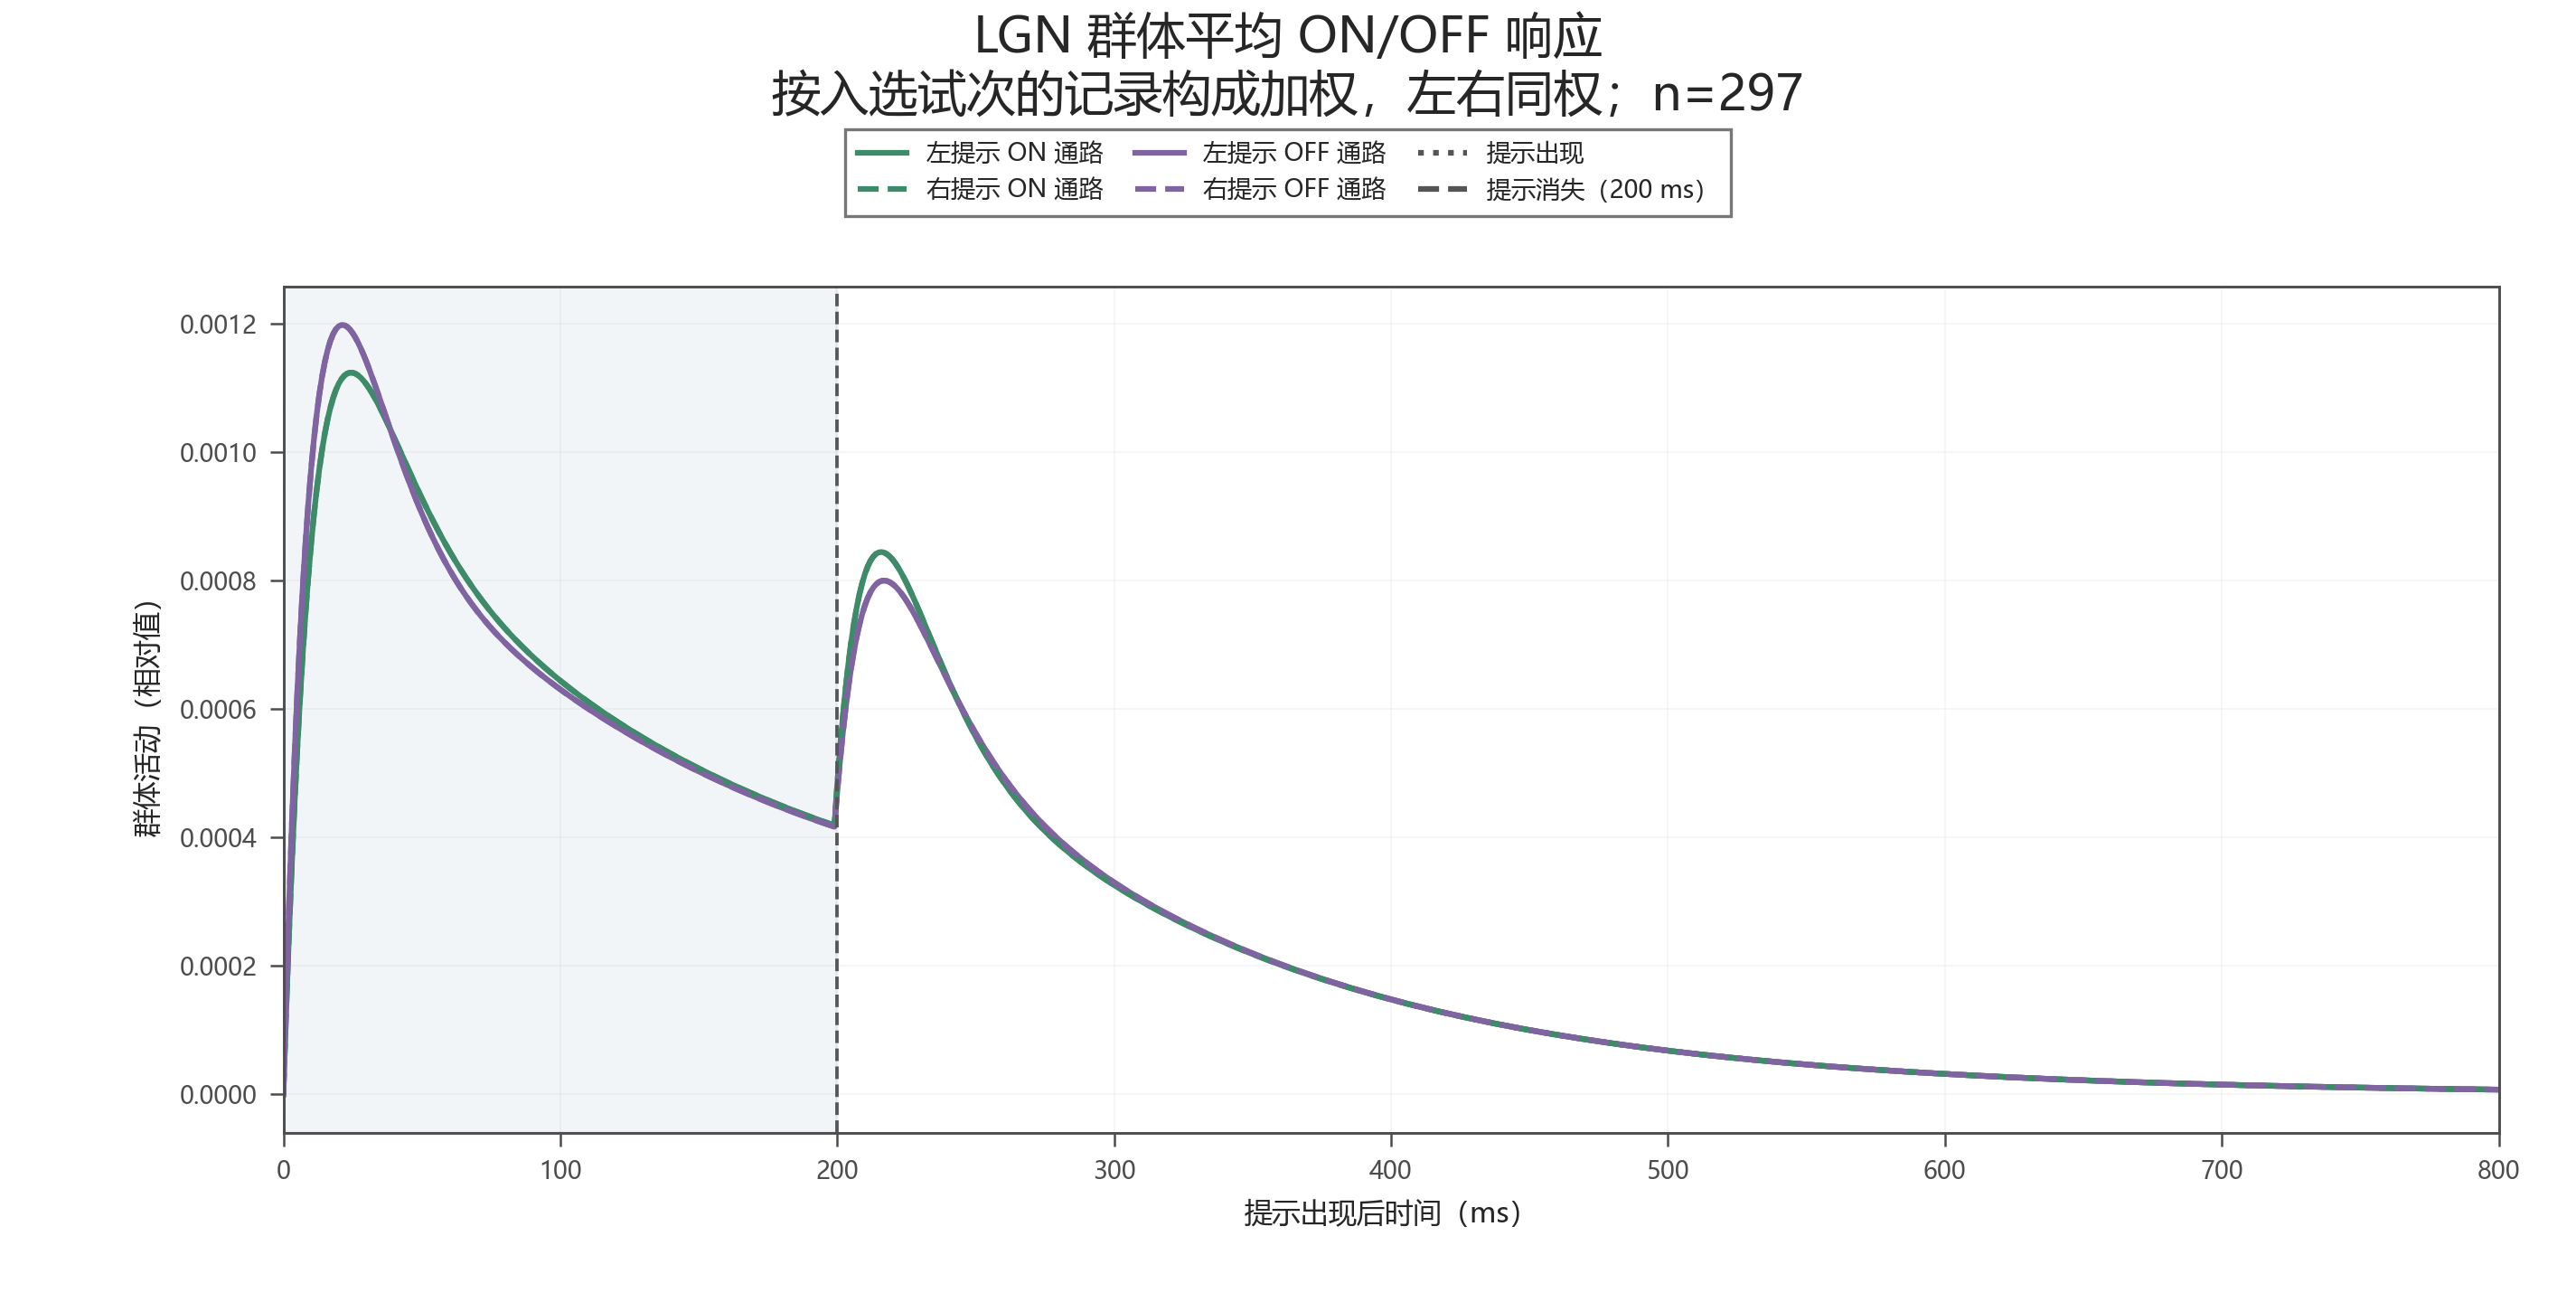
\includegraphics[width=0.96\textwidth]{src/C/q2/output/final_pic/LGN平均响应.png}
\caption{LGN 群体平均 ON/OFF 响应。实线和虚线分别表示左右提示；竖线标出提示出现与 200 ms 提示消失，曲线幅值为相对活动量。}\label{fig:q2_lgn_mean}
\end{figure}

\begin{figure}[H]
\centering
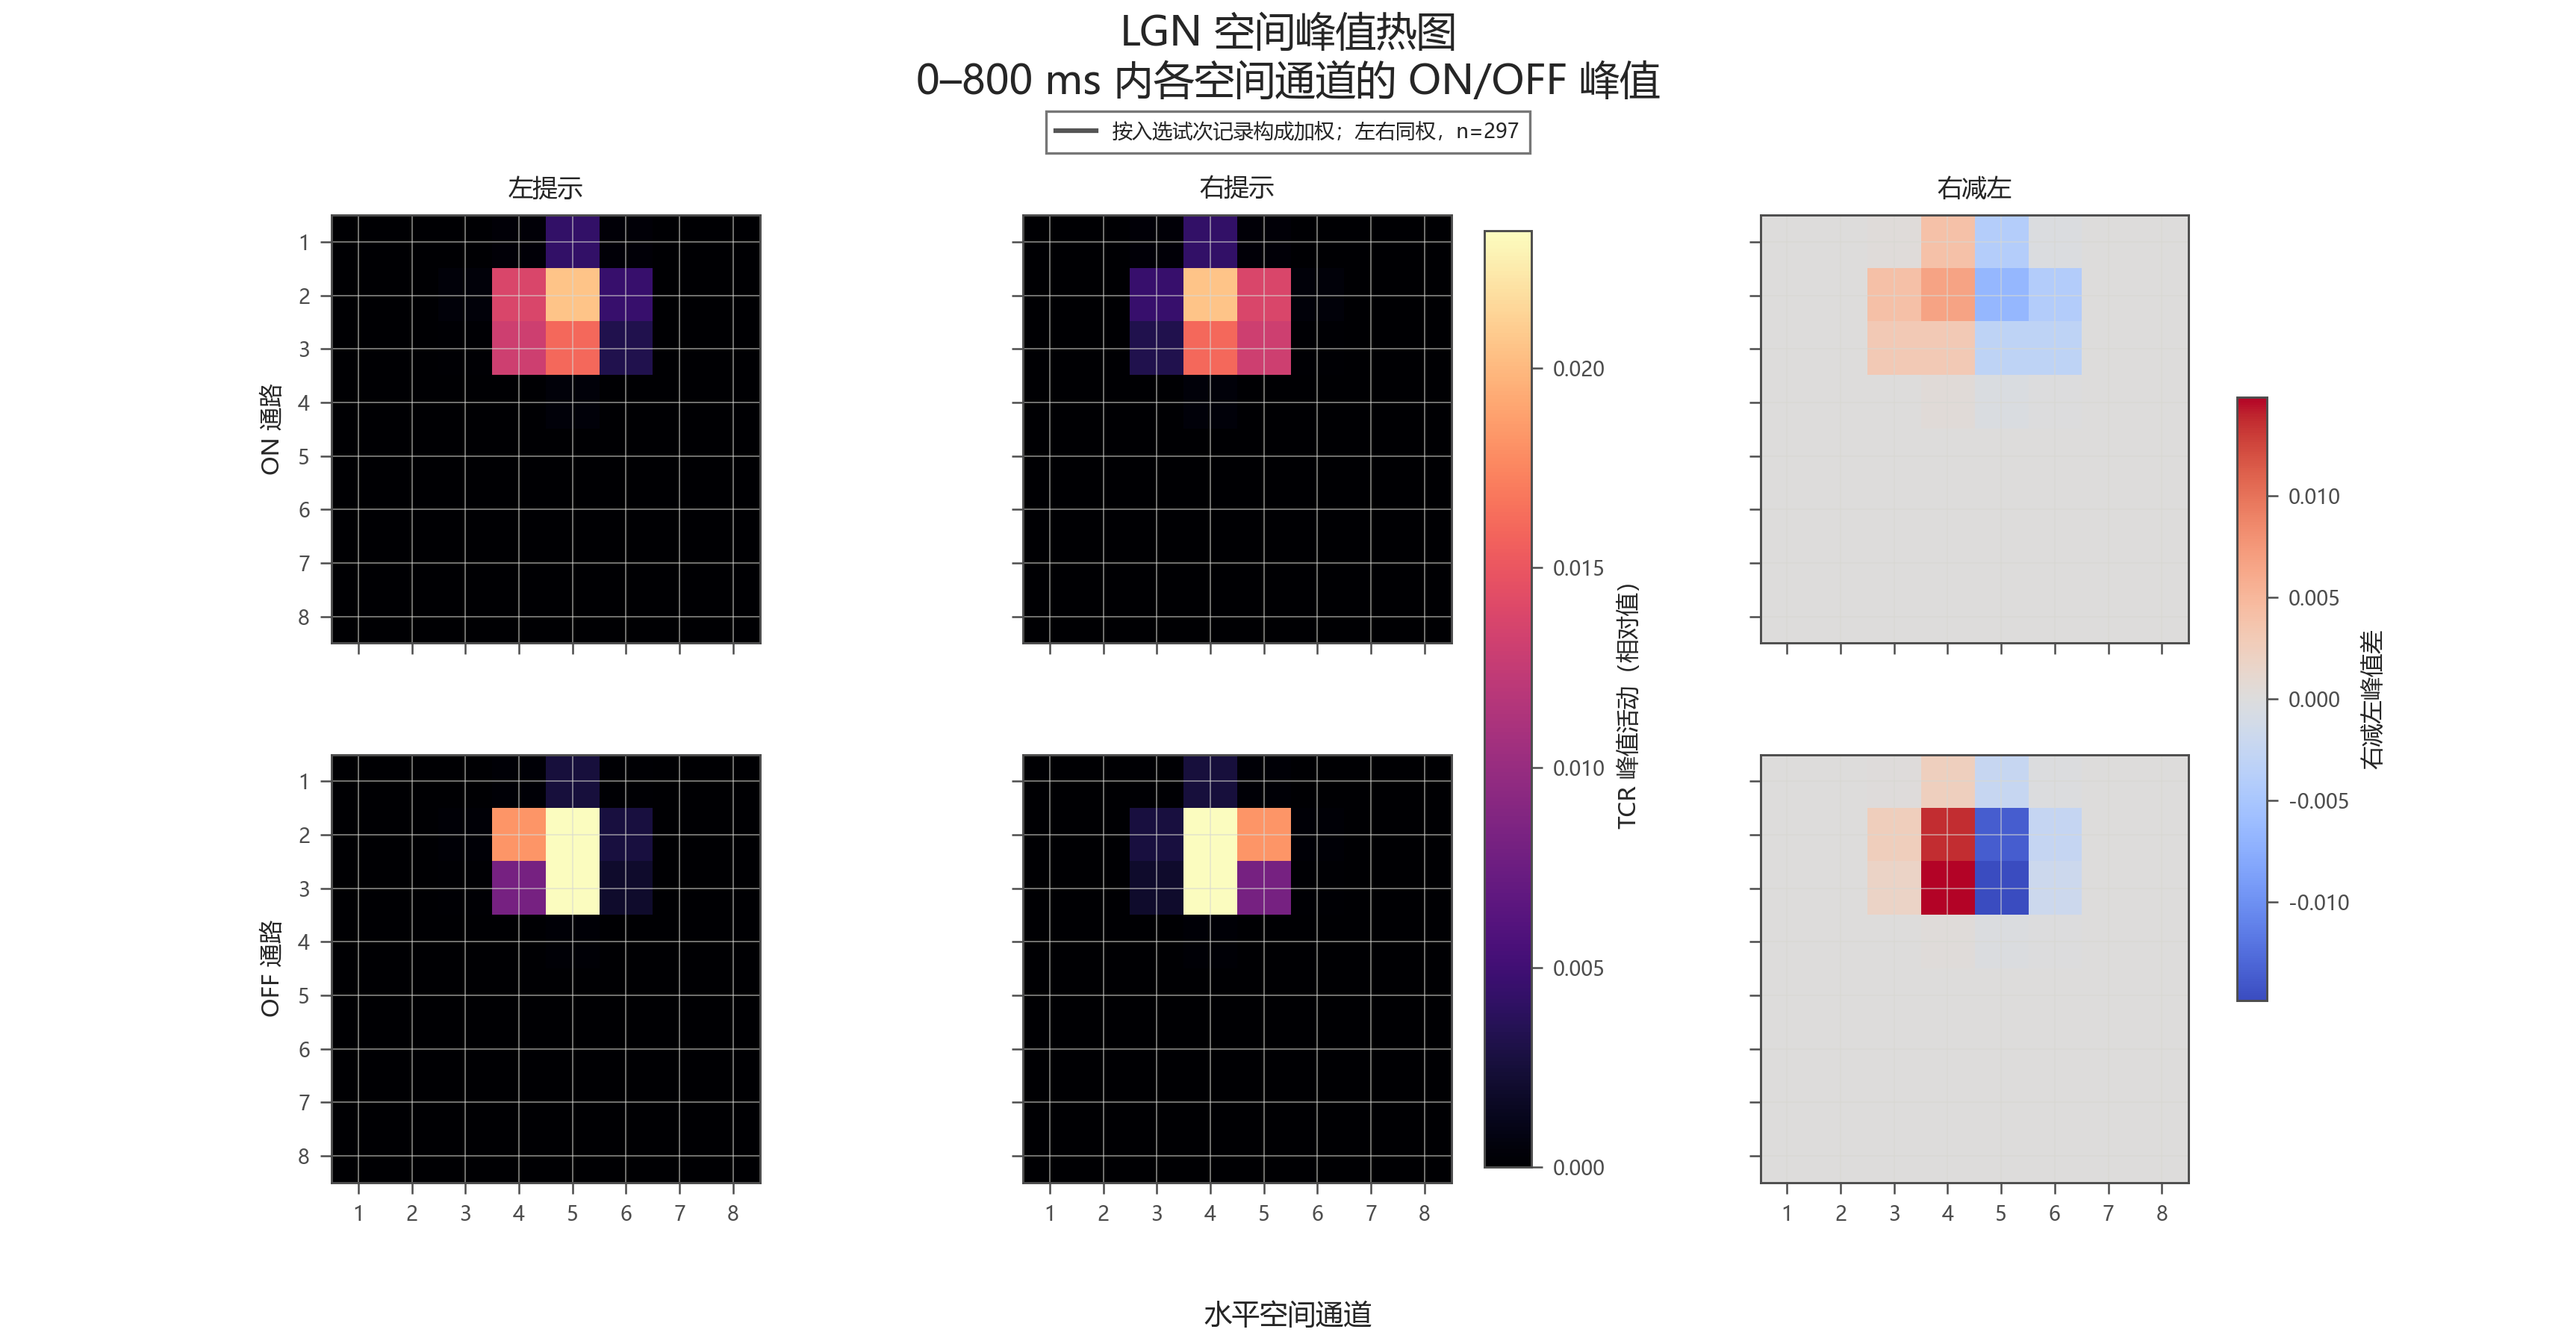
\includegraphics[width=0.96\textwidth]{src/C/q2/output/final_pic/LGN空间峰值热图.png}
\caption{LGN 空间峰值热图。上、下两行为 ON、OFF 通路；三列为左提示、右提示及右减左差异，颜色表示 0--800 ms 内各 TCR 空间通道的峰值活动或峰值差。}\label{fig:q2_lgn_peaks}
\end{figure}

\subsubsection{Gabor 方向与三角构型编码}

令 \(S=R_{\rm ON}-R_{\rm OFF}\) 为有符号中继图。为保留三角边缘朝向，模型计算 \(0^\circ\)、\(45^\circ\)、\(90^\circ\) 和 \(135^\circ\) 四个方向的偶、奇 Gabor 响应并合成为方向能量：

\begin{equation}
V_\theta(x,y,t)=\sqrt{(K^e_\theta*S)^2+(K^o_\theta*S)^2},\qquad
B(x,y,t)=\frac{1}{2}\sqrt{\sum_\theta V_\theta(x,y,t)^2}.
\end{equation}

Gabor 响应由局部方向滤波得到，方向滤波的建模动机参见 Gabor 的时频局部化分析\cite{gabor1946}。为表达边、角与整体排列的共同出现，左右三角模板分别沿三条边和三个顶点设置支持位置；局部响应经平滑后以等权几何汇总形成 \(H_L,H_R\)。模板偏好通道取三角中心邻域响应差的正部：

\begin{equation}
d_L(t)=[r_L(t)-r_R(t)]_+,\qquad d_R(t)=[r_R(t)-r_L(t)]_+.
\end{equation}

这里的 L/R 分别表示左、右模板偏好。实现将空间图按 \(8\times8\) 池化，前端特征每 4 ms 计算一次，再插值到 1 ms 群体动力学网格。图~\ref{fig:q2_io} 把实际数据、群体状态、五个源代理和传感器输出放在同一计算链中；其中模型状态是确定性前向模拟，实测输入来自留出记录折。

图~\ref{fig:q2_gabor_difference} 展示四个方向通道的空间响应差，颜色表示右提示减左提示；图~\ref{fig:q2_gabor_spatial} 则把左右提示按方向分别展示。两图使用相同的 297 个提示试次构成对各记录模型响应加权，表示的是模型内部方向/位置特征，不是 EEG。空间响应热图为了可读性将原生 \(8\times8\) 通道按相邻 \(2\times2\) 区域取均值显示为 \(4\times4\) 数值矩阵；差异图保留原生通道分辨率。

\begin{figure}[H]
\centering
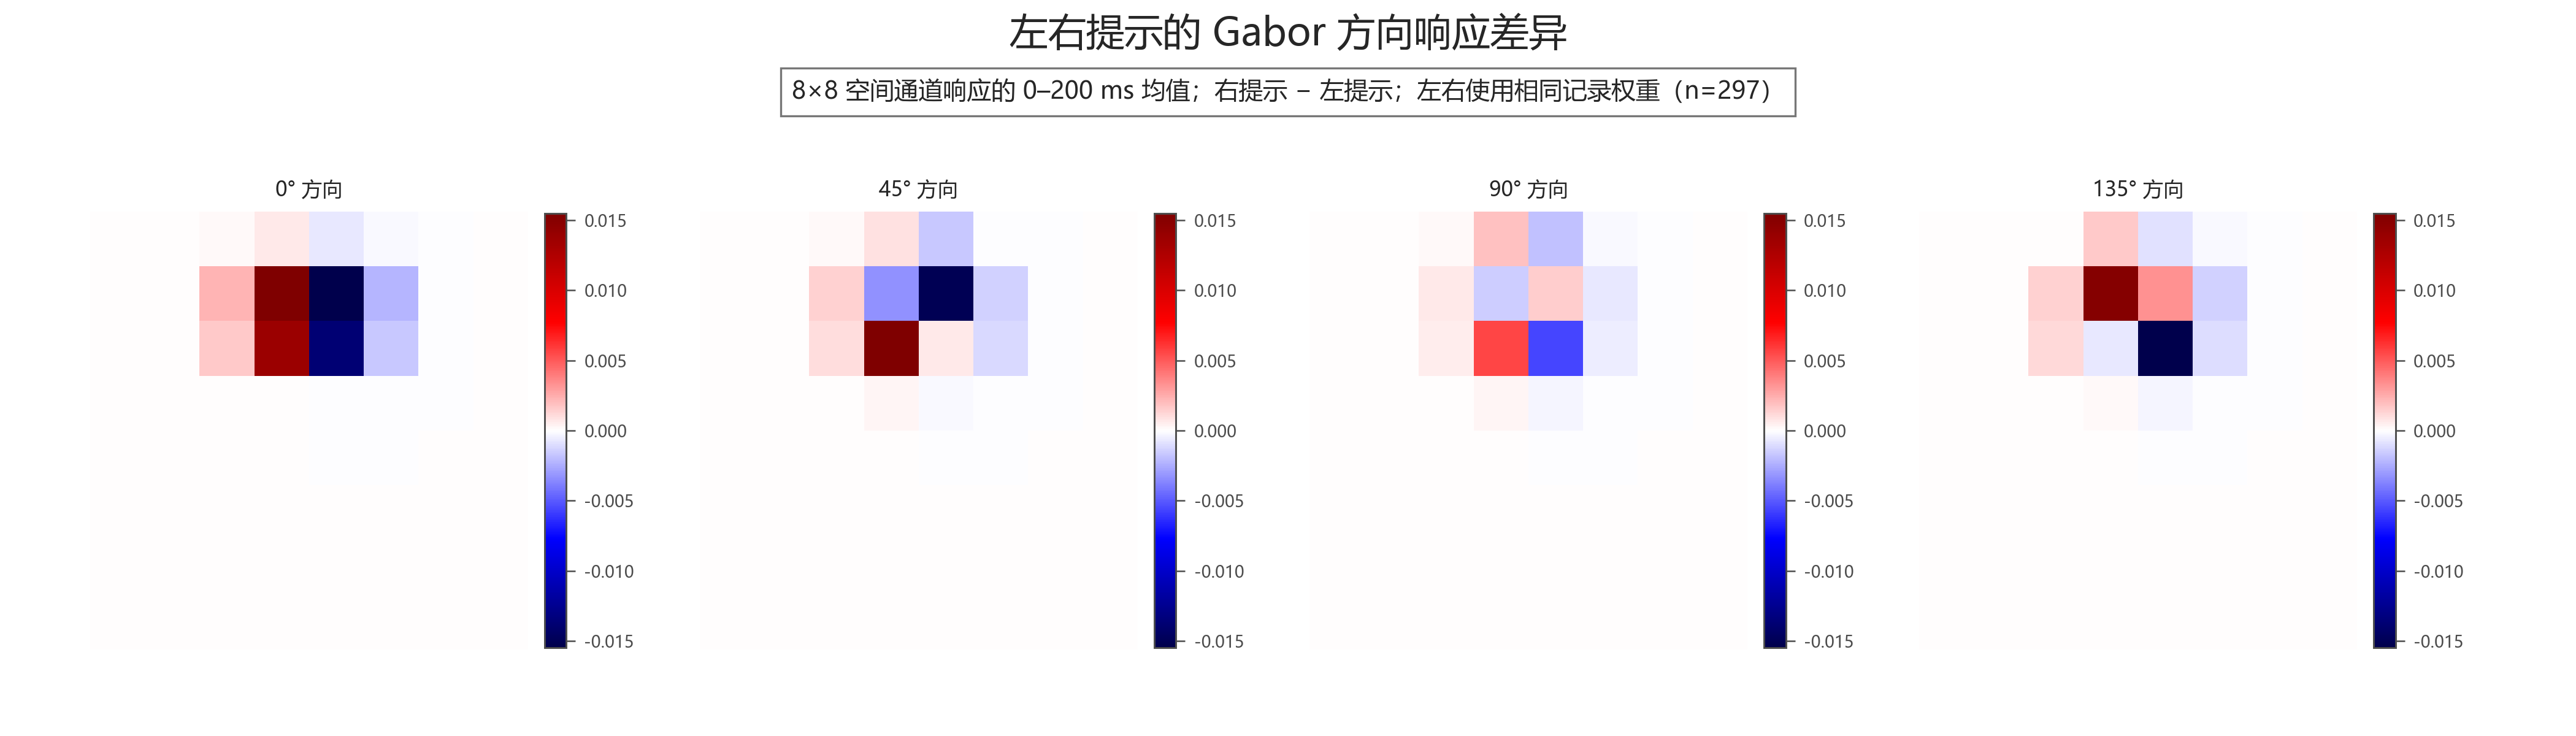
\includegraphics[width=0.96\textwidth]{src/C/q2/output/final_pic/Gabor左右差异图.png}
\caption{左右提示的 Gabor 方向响应差异。各面板对应一个方向；红、蓝分别表示右提示响应高于、低于左提示响应，差值为提示显示期 0--200 ms 的时间均值。}\label{fig:q2_gabor_difference}
\end{figure}

\begin{figure}[H]
\centering
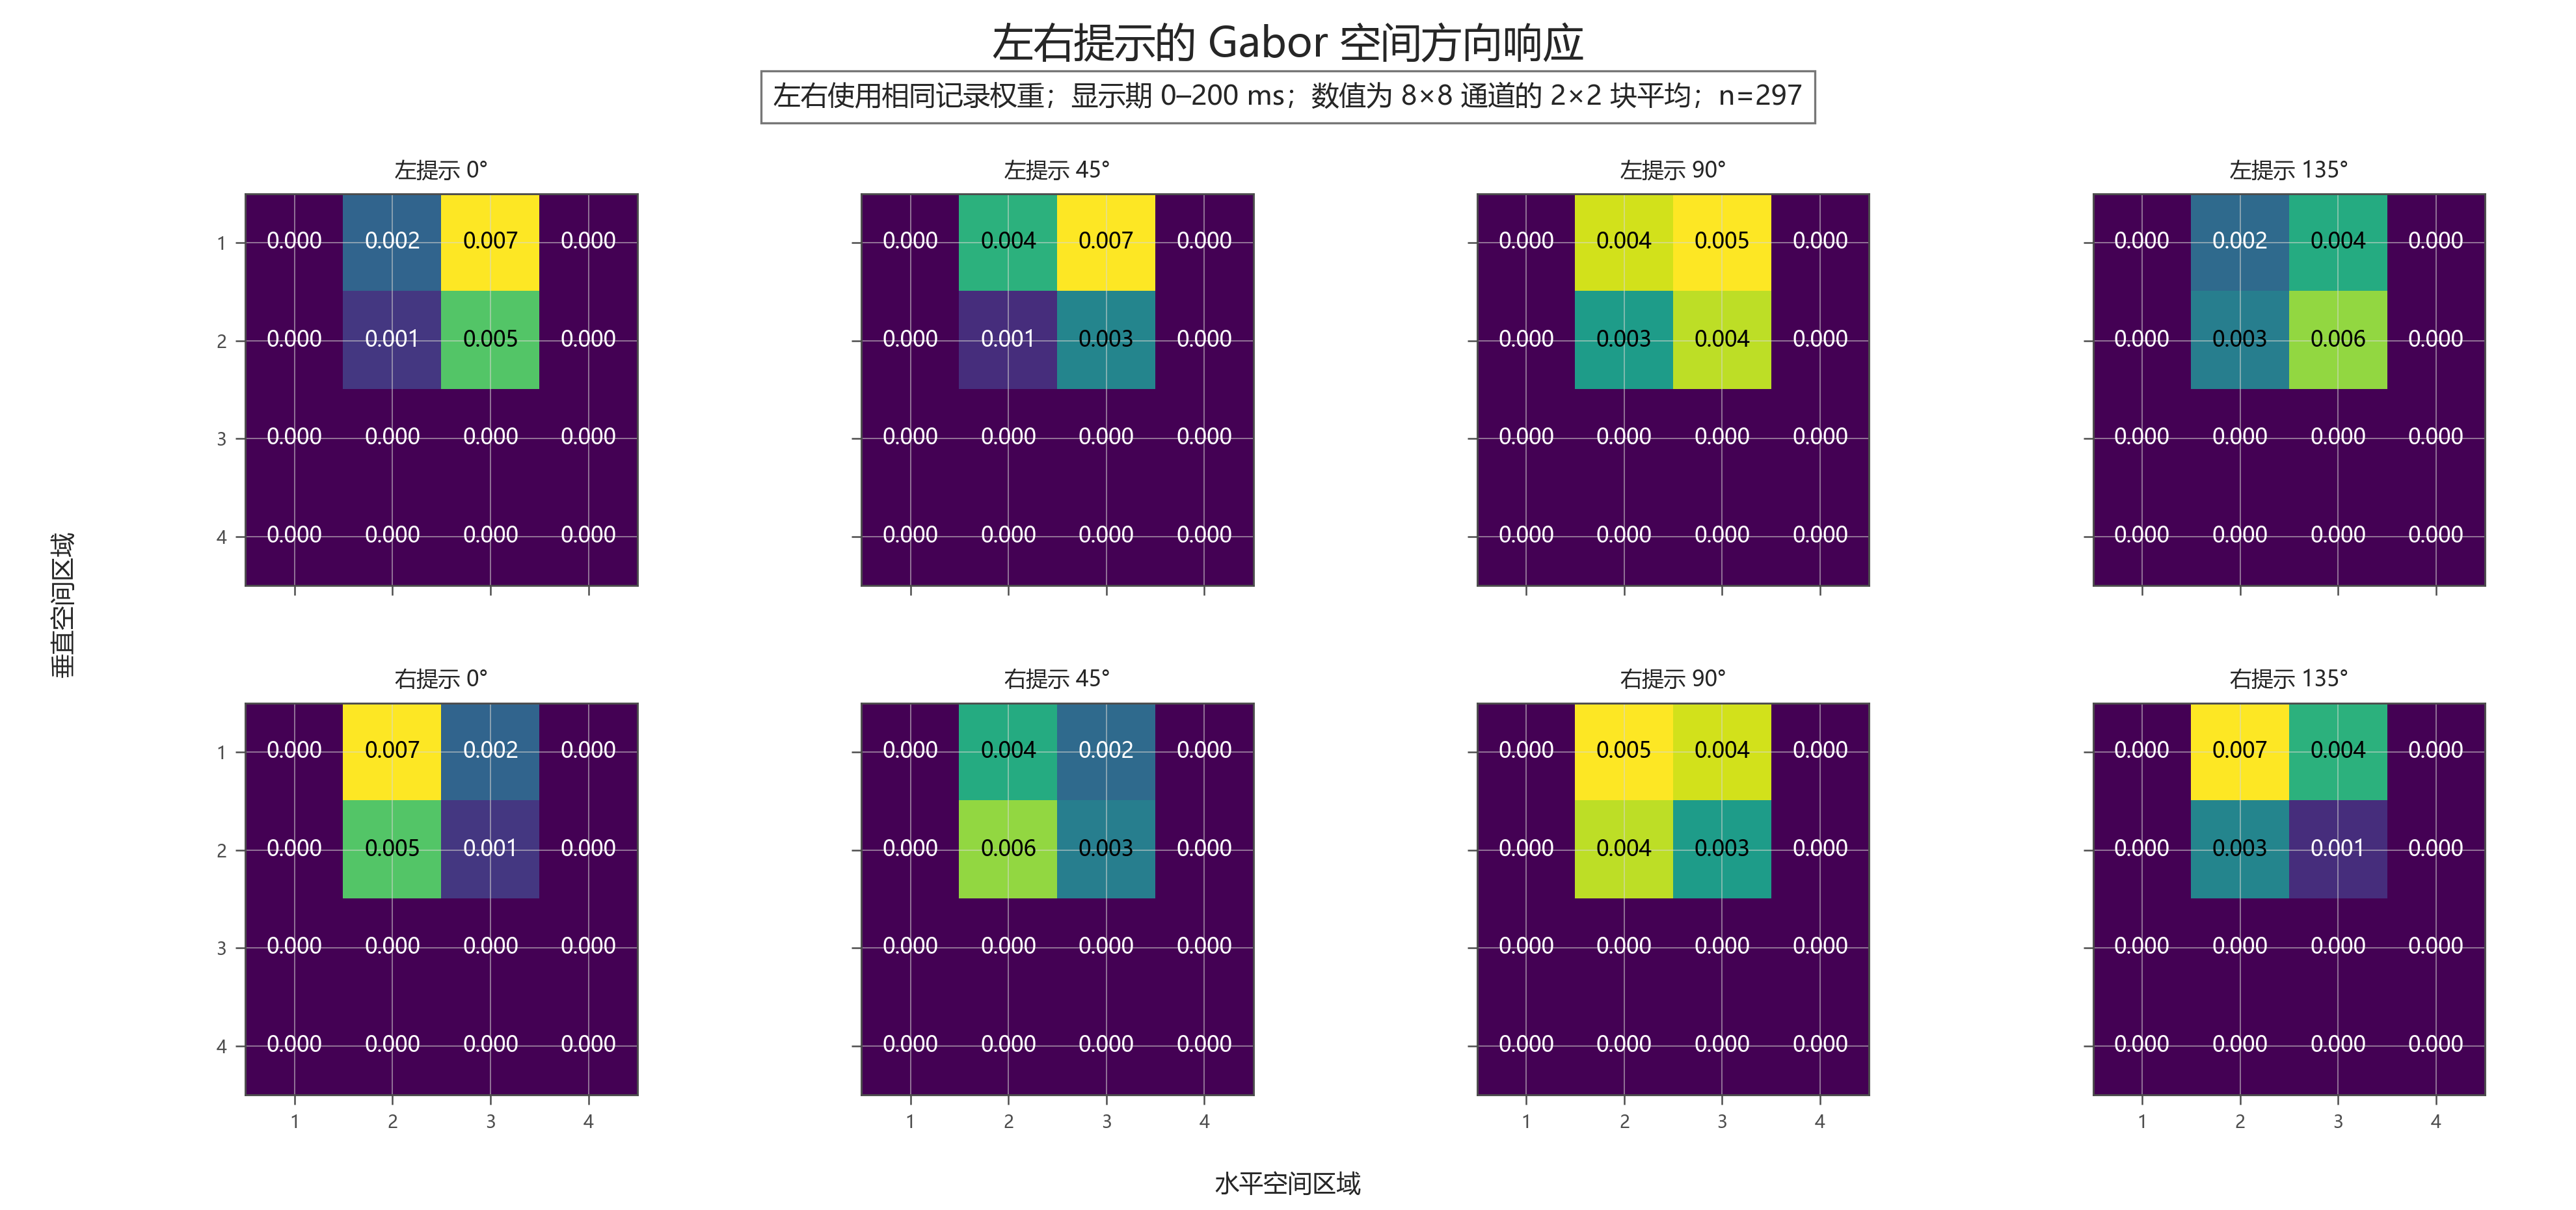
\includegraphics[width=0.96\textwidth]{src/C/q2/output/final_pic/Gabor空间响应热图.png}
\caption{左右提示的 Gabor 空间方向响应。行表示提示方向，列表示滤波方向；每个数值为原生 \(8\times8\) 空间通道相邻 \(2\times2\) 块的均值，四个方向分别展示而未合并；同一方向下左右使用相同色标，不同方向之间不比较颜色幅度。}\label{fig:q2_gabor_spatial}
\end{figure}

\begin{figure}[H]
\centering
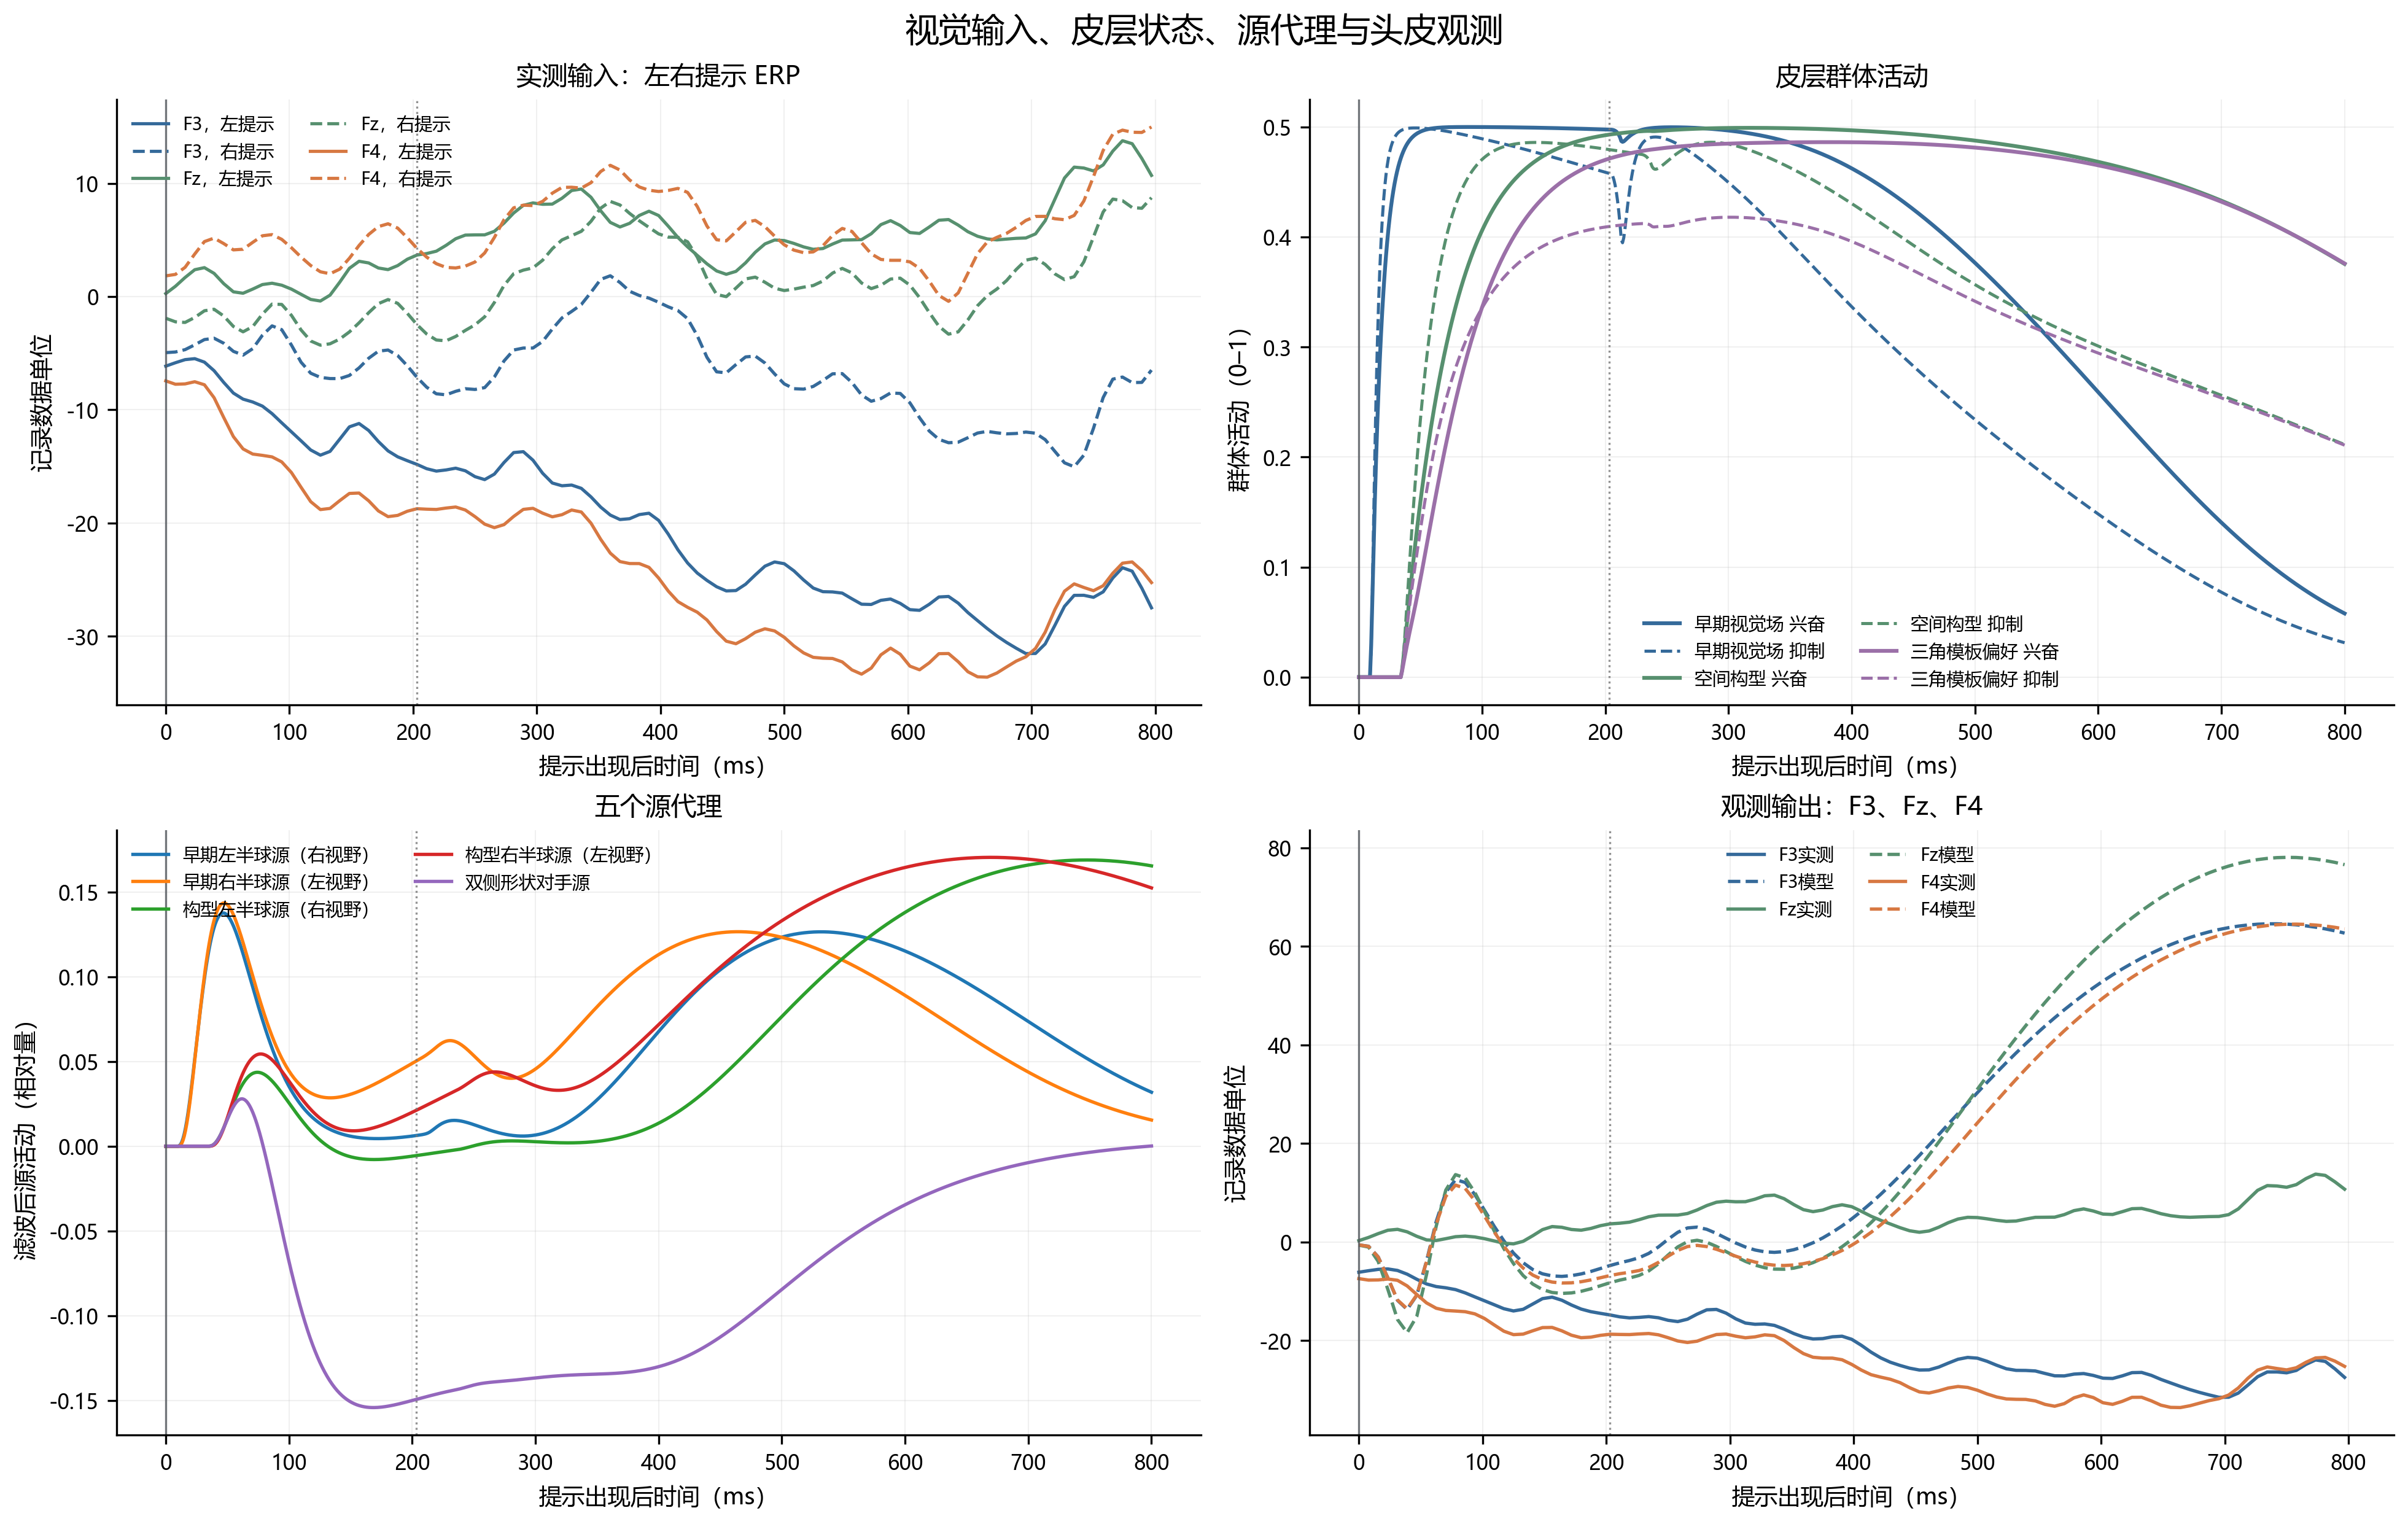
\includegraphics[width=0.96\textwidth]{src/C/q2/documents/figures/revision_v3_真实数据与皮层观测模块IO.png}
\caption{视觉输入、皮层状态、源代理与头皮观测}\label{fig:q2_io}
\end{figure}

\subsubsection{三组兴奋-抑制群体动力学}

前端特征投影为三组左右通道：早期视觉组接收 \(B\) 的左右视野均值，空间构型组接收 \(H_L+H_R\) 的左右视野均值，模板偏好组接收 \(d_L,d_R\)。早期组向空间构型组传递视野对应活动；模板偏好组的两个通道共同接收左右早期活动的等权平均，避免将模板偏好误当作视野或半球标签。

兴奋和抑制状态采用 Wilson-Cowan 型群体方程\cite{wilsonCowan1972}：

\begin{equation}
\begin{aligned}
J^E_{p,c}&=w_{EE}E_{p,c}-g_iw_{EI}I_{p,c}+g_Pu_{p,c}+F^E_{p,c},\\
J^I_{p,c}&=w_{IE}E_{p,c}-w_{II}I_{p,c}+g_Qu_{p,c}+F^I_{p,c},\\
\tau^E_p\dot E_{p,c}&=-E_{p,c}+(1-E_{p,c})\Phi_{5,0.35}(J^E_{p,c}),\\
\tau^I_p\dot I_{p,c}&=-I_{p,c}+(1-I_{p,c})\Phi_{5,0.35}(J^I_{p,c}).
\end{aligned}
\end{equation}

其中 \(p\) 依次表示早期、构型和模板偏好群体，\(c\in\{L,R\}\)；\(u_{p,c}\) 为归一化视觉输入，\(F^E,F^I\) 为前馈项。所有状态从 0 初始化，以 1 ms 显式 Euler 递推并限制在 \([0,1]\)。固定耦合参数为 \(w_{EE}=1.4,w_{EI}=1.1,w_{IE}=1.0,w_{II}=0.8,g_P=2.2,g_Q=1.2\)；早期组 \(\tau_E=18\) ms、\(\tau_I=10\) ms、输入延迟 8 ms。后两组使用 \(\tau_E=\tau_s,\tau_I=0.55\tau_s\)，前馈延迟 33 ms，兴奋和抑制前馈系数分别为 0.9 和 0.45。三类输入尺度由左右标准提示的 0 至 200 ms 视觉驱动预先计算，未使用留出 EEG 估计。

图~\ref{fig:q2_cortical_differences} 给出左右提示驱动下三组群体的兴奋、抑制活动差。左右输入使用同一组记录内拟合参数，并按相同的记录权重聚合。早期视觉组和空间构型组的两个通道对应左右视野；第三组的两个通道表示左右三角模板偏好，不能解释为左右半球。图中显示的是模型状态之差而非 EEG；它用于追踪空间与模板输入如何经群体动力学形成左右差异。

\begin{figure}[H]
\centering
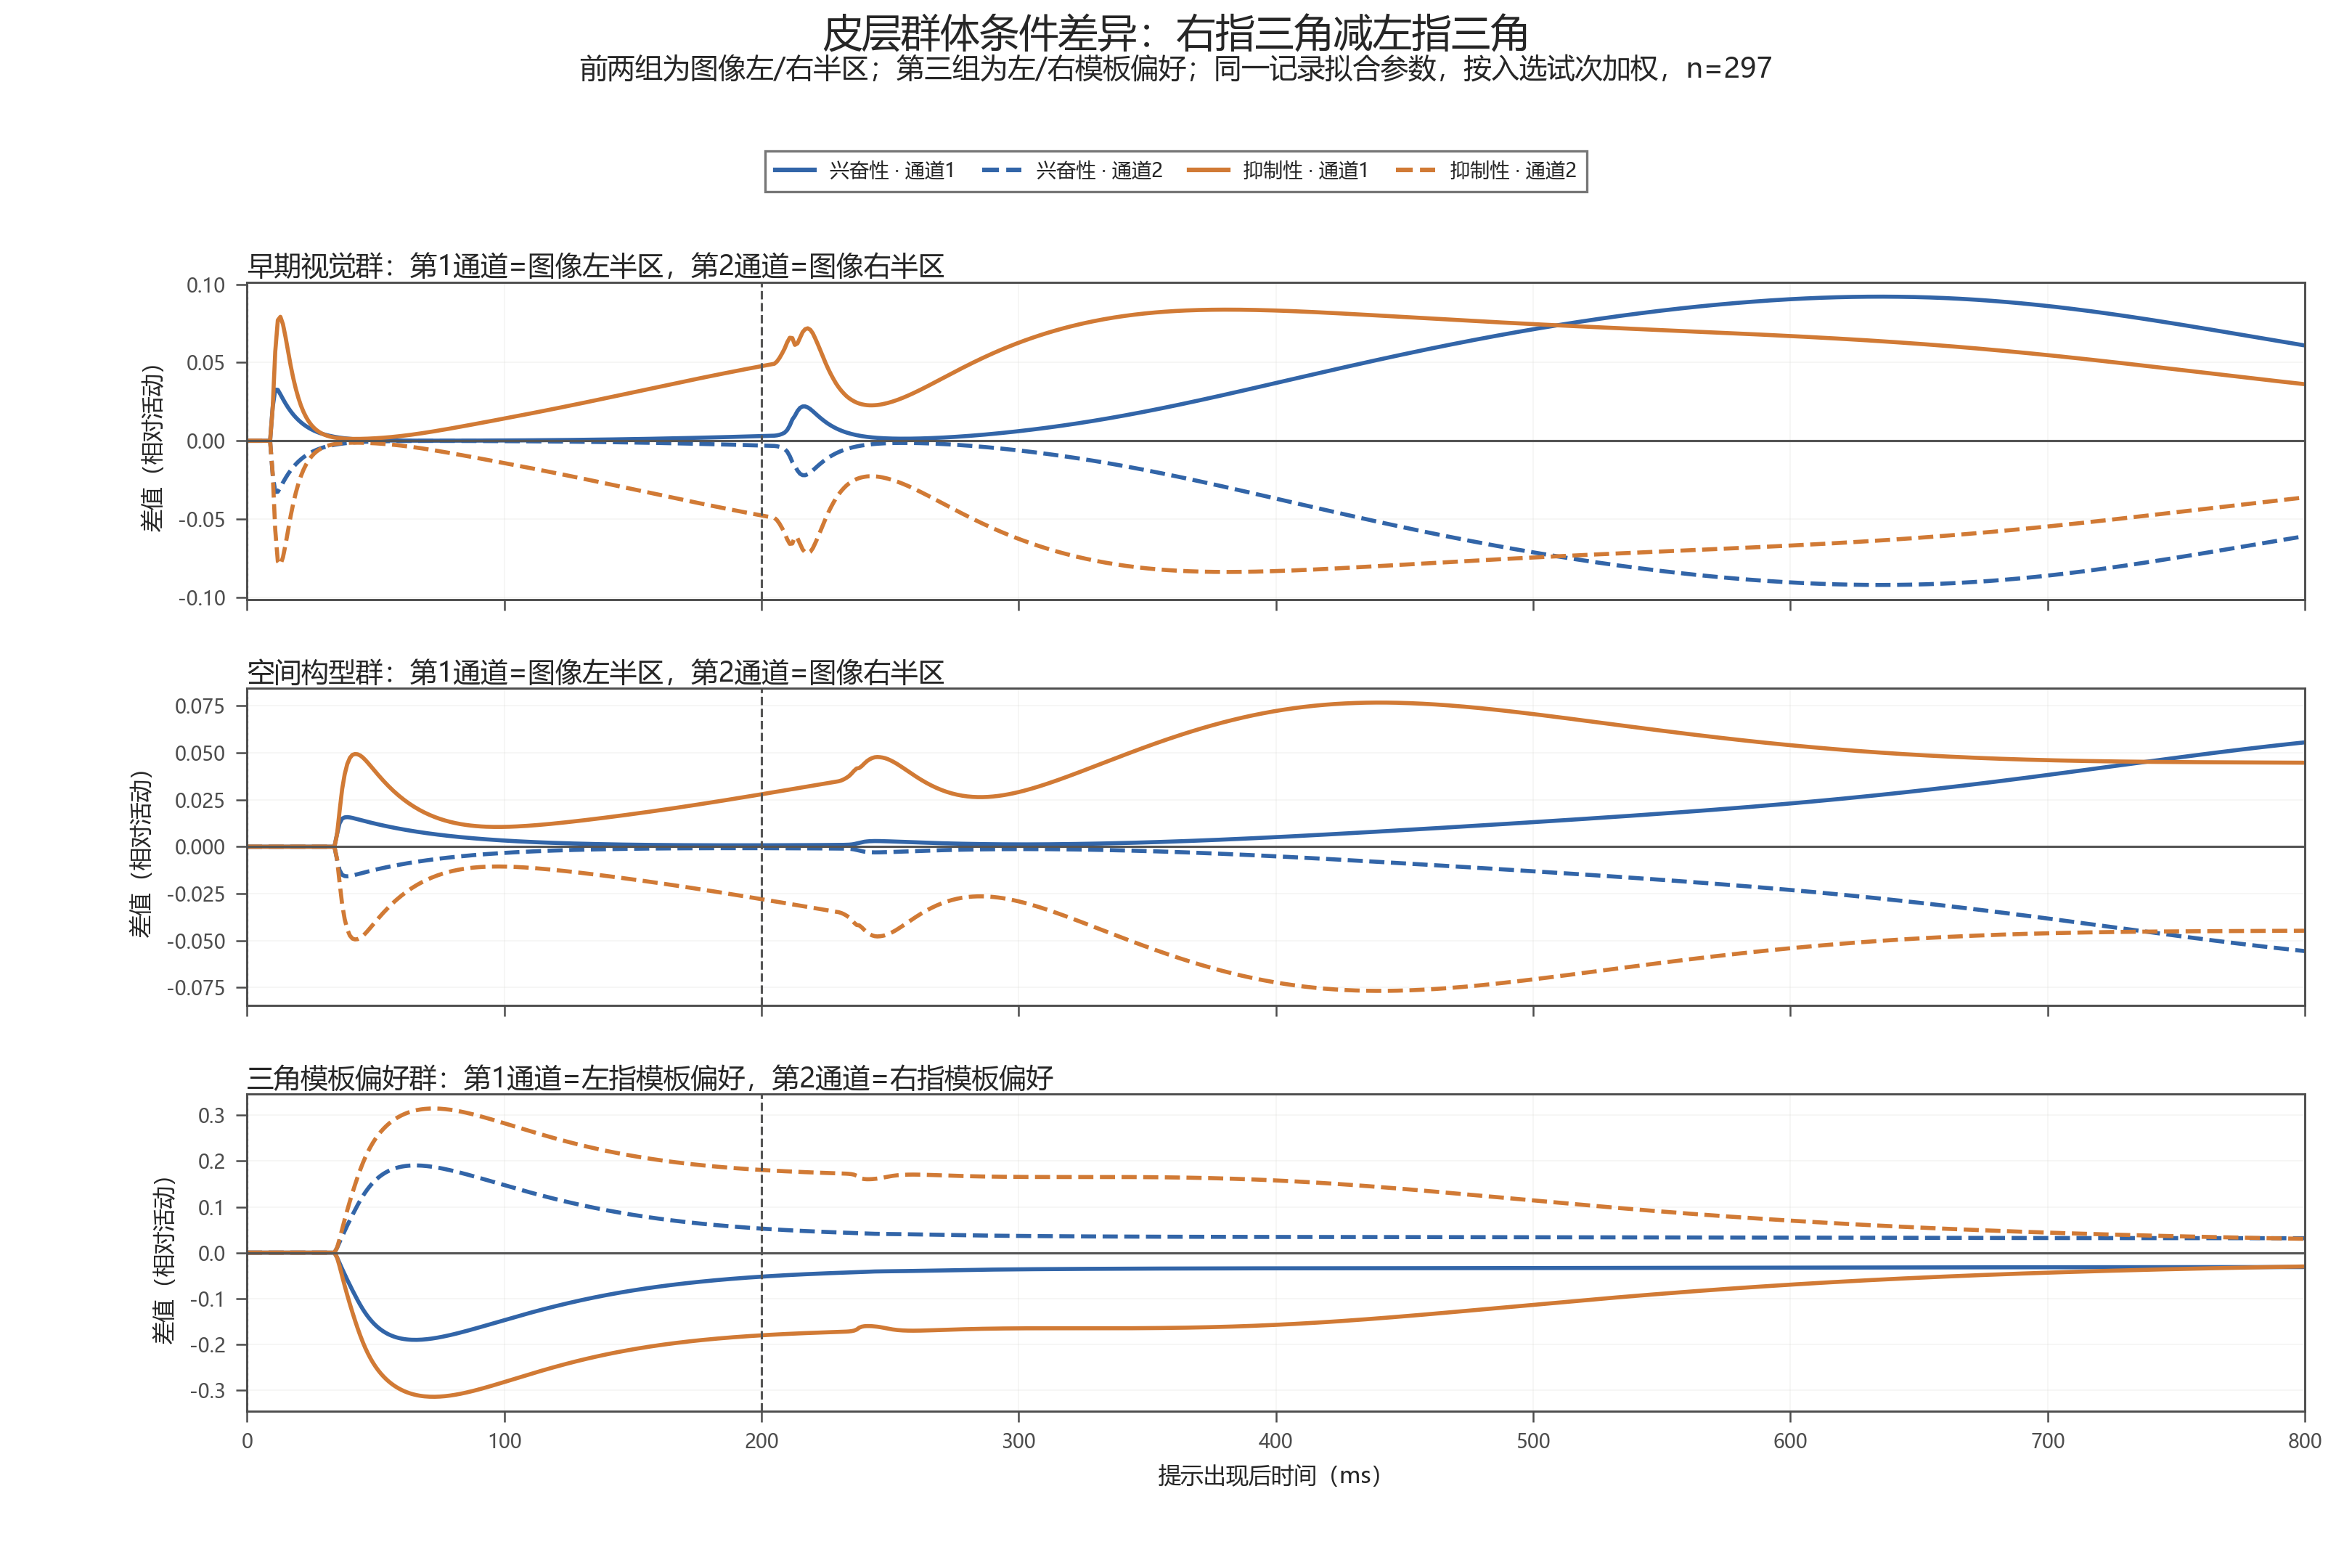
\includegraphics[width=0.96\textwidth]{src/C/q2/output/final_pic/皮层条件差异诊断图.png}
\caption{三组皮层功能群体的右提示减左提示响应差。每组分别显示兴奋性和抑制性状态；通道含义按群体定义区分，模板偏好通道不代表半球位置。}\label{fig:q2_cortical_differences}
\end{figure}

\subsubsection{五源代理与头皮正向映射}

为将群体状态转为可观测的候选电流代理，对兴奋和抑制活动分别施加因果突触核并作差：

\begin{equation}
h_\tau(t)=\frac{t e^{-t/\tau}}{\tau^2},\quad t\ge0,\qquad
P_{p,c}(t)=(h_{10}*E_{p,c})(t)-(h_{20}*I_{p,c})(t).
\end{equation}

离散核按步长归一化。前两组分别按对侧视野路由至左右半球位置代理；模板偏好差形成一个双侧中线对手代理：

\begin{equation}
\mathbf q(t)=\left[
P_{\rm early,RVF\to LH},P_{\rm early,LVF\to RH},
P_{\rm config,RVF\to LH},P_{\rm config,LVF\to RH},
P_{\rm preference,L}-P_{\rm preference,R}
\right]^{\mathsf T}.
\end{equation}

其中 RVF、LVF 分别表示右、左视野，LH、RH 表示模型中的左、右半球位置标签。第五项表示双侧模板对手量。五项均为功能源代理。

电极和双乳突参考点投影到半径 \(90\) mm 的外表面，内部源位置和径向方向按规范坐标固定，导电率取 \(\sigma=0.33\) S/m。均匀无限导体点偶极近似下，电极 \(e\) 对源 \(j\) 的系数为

\begin{equation}
L_{ej}=\frac{\mathbf n_j^{\mathsf T}(\mathbf r_e-\mathbf r_j)}
{4\pi\sigma\lVert\mathbf r_e-\mathbf r_j\rVert^3},\qquad
G_{ej}=L_{ej}-\frac{L_{M_1j}+L_{M_2j}}{2},\qquad
\mathbf y_{\rm model}(t)=\mathbf G\mathbf q(t).
\end{equation}

实现采用的 \(3\times5\) 矩阵按 F3、Fz、F4 为行，按上述源顺序为列：

\begin{equation}
\mathbf G\approx\begin{bmatrix}
0.661&0.961&-2.688&-4.365&-0.330\\
1.101&1.101&-4.299&-4.299&-0.489\\
0.961&0.661&-4.365&-2.688&-0.330
\end{bmatrix}.
\end{equation}

该矩阵给出固定的正向近似。源代理没有以 \(\mathrm{A\,m}\) 标定，参考电极和个体头部组织也未由受试者影像确定，因此最终传感器曲线按相对单位报告，不换算为微伏或脑区定位结论。

图~\ref{fig:q2_leadfield} 将同一 \(3\times5\) 固定映射以热图表示，行是观测电极，列是功能源代理，数字是矩阵系数。该图便于核对源对各电极的相对权重和左右镜像结构；系数来自规范坐标下的均匀无限导体点偶极近似，源电流代理未标定为物理偶极矩，故不能将颜色或数值直接解释为真实 EEG 的微伏贡献。

\begin{figure}[H]
\centering
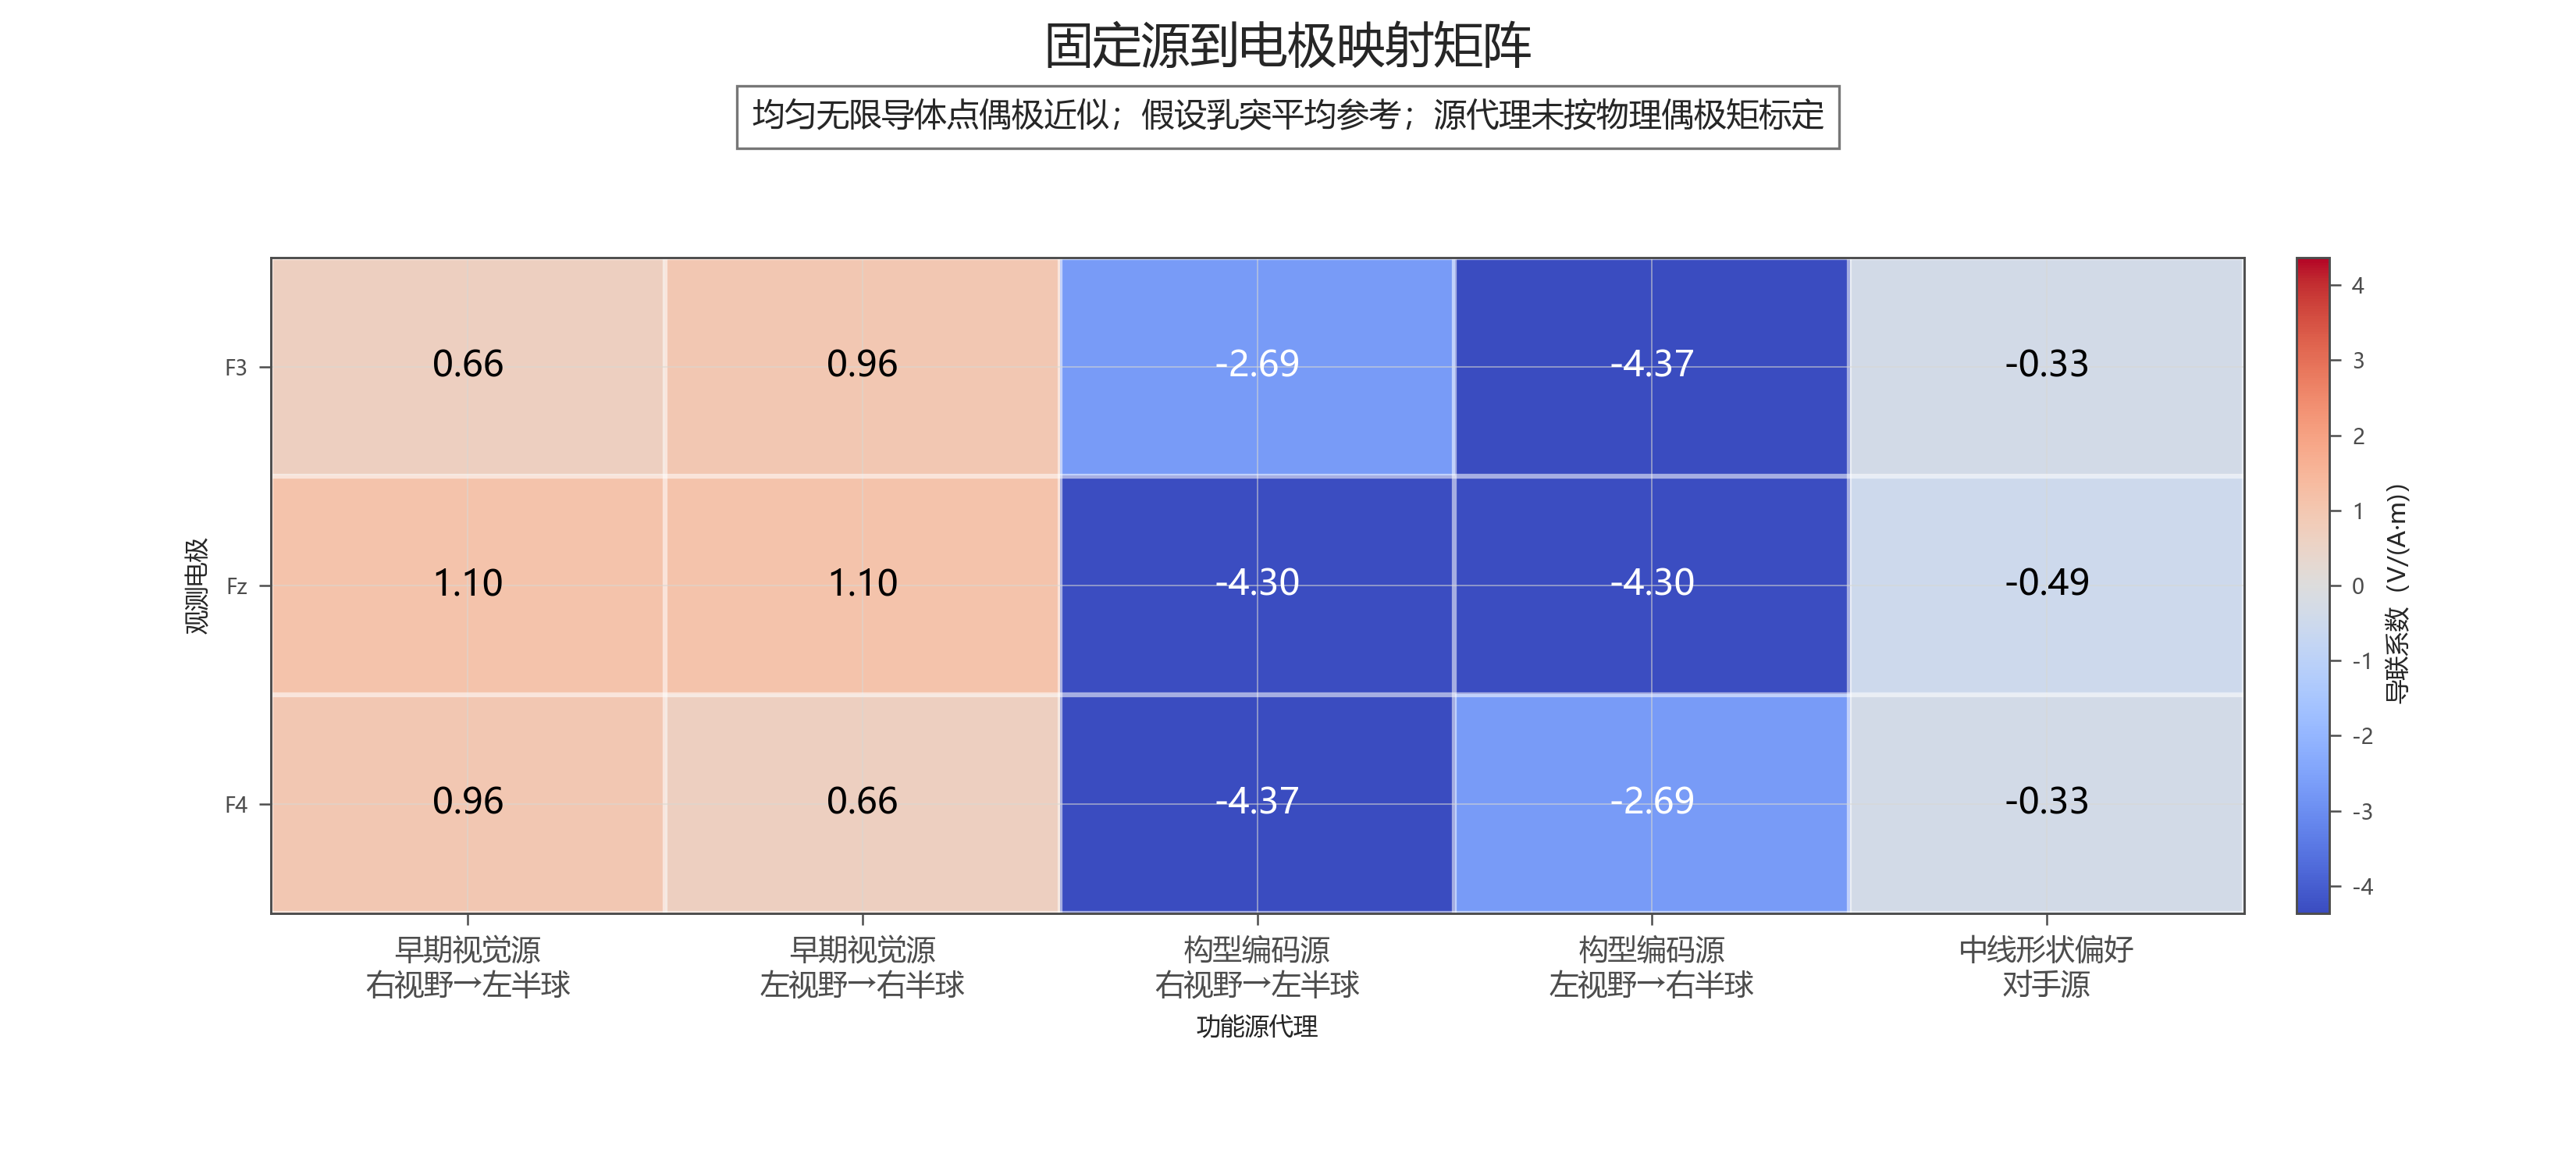
\includegraphics[width=0.92\textwidth]{src/C/q2/output/final_pic/简化导联矩阵热图.png}
\caption{固定源到电极映射矩阵。行对应 F3、Fz、F4，列对应四个按对侧视野路由的早期/构型源和一个双侧中线形状偏好对手源；数值为点偶极近似下的导联系数。}\label{fig:q2_leadfield}
\end{figure}

\subsection{参数估计与验证设计}

模型从提示起点连续模拟至 3000 ms，将信号嵌入完整 \([-1,3]\) s 试次后统一处理。模拟曲线和第一问清洗数据采用一致的四阶 \(0.2\)--\(24\) Hz Butterworth 零相位滤波、\(256\) Hz 至 \(128\) Hz 重采样及 \([-200,0)\) ms 逐通道基线校正；比较窗裁至 \(0\) 至 \(796.875\) ms。真实记录的完整试次可能含约 2.2 s 目标事件，而本模型只模拟提示输入；比较窗落在提示事件范围内，因此该事件上下文差异不参与波形比较，但仍作为解释限制列出。

模型参数仅使用 Stage1 左右条件平均 ERP 估计。每折留出一份完整 MAT 记录，其余三份记录训练；左、右条件共用 \(\tau_s,g_i,\tau_a\) 和一个有符号增益 \(\alpha\)。\(\tau_a\) 按七点网格剖面搜索，\(\tau_s\in[20,100]\) ms、\(g_i\in[0.5,1.5]\) 由有界 L-BFGS-B 搜索。对训练记录 \(r\) 和提示条件 \(c\)，增益通过最小二乘闭式解给定：

\begin{equation}
\alpha^*=\frac{\sum_{r,c}w_{r,c}\langle\widehat{\mathbf Y}_{r,c},\mathbf Y_{r,c}\rangle}
{\sum_{r,c}w_{r,c}\lVert\widehat{\mathbf Y}_{r,c}\rVert_F^2},\qquad
\mathcal L=\sum_{r,c}w_{r,c}\operatorname{MSE}\!\left(\mathbf Y_{r,c}-\alpha^*\widehat{\mathbf Y}_{r,c}\right),
\end{equation}

其中记录和左右条件等权，\(\mathbf Y\) 为实测平均 ERP，\(\widehat{\mathbf Y}\) 为未缩放模型曲线。拟合参数描述当前搜索的最优候选；若优化器未报告收敛，不解释为识别出的生理参数。

留出 ERP 以 \(\mathrm{NRMSE}=\mathrm{RMSE}/\sqrt{\operatorname{mean}(Y^2)}\) 评价，左右差异波相关用于比较预测和观测形状。三电极差异还投影到共同、侧化、形状三个正交模式：

\begin{equation}
u_0=\frac{F3+Fz+F4}{\sqrt3},\qquad
u_1=\frac{F4-F3}{\sqrt2},\qquad
u_2=\frac{F3-2Fz+F4}{\sqrt6}.
\end{equation}

左右特征表示直接从真实单试次 EEG 提取。对 \(W_1=[100,250)\) ms、\(W_2=[250,500)\) ms、\(W_3=[500,800)\) ms，计算三个电极各自的窗口均值并按电极顺序拼接：

\begin{equation}
\mathbf z=\left[
\bar y_{F3,W_1},\bar y_{Fz,W_1},\bar y_{F4,W_1},
\bar y_{F3,W_2},\bar y_{Fz,W_2},\bar y_{F4,W_2},
\bar y_{F3,W_3},\bar y_{Fz,W_3},\bar y_{F4,W_3}
\right]^{\mathsf T}\in\mathbb R^9.
\end{equation}

图~\ref{fig:q2_mode_feature_differences} 另给出共同、侧化和中央--两侧三个观测模式的记录内右减左差异。该补充图使用 \([80,200)\)、\([250,450)\)、\([450,700)\) ms 三个窗口，并以 2000 次试次重采样估计区间；它与上式主分类特征的电极分量及窗口定义不同，不用于表 6 的留一记录分类，也不据此宣称统计显著。

\begin{figure}[H]
\centering
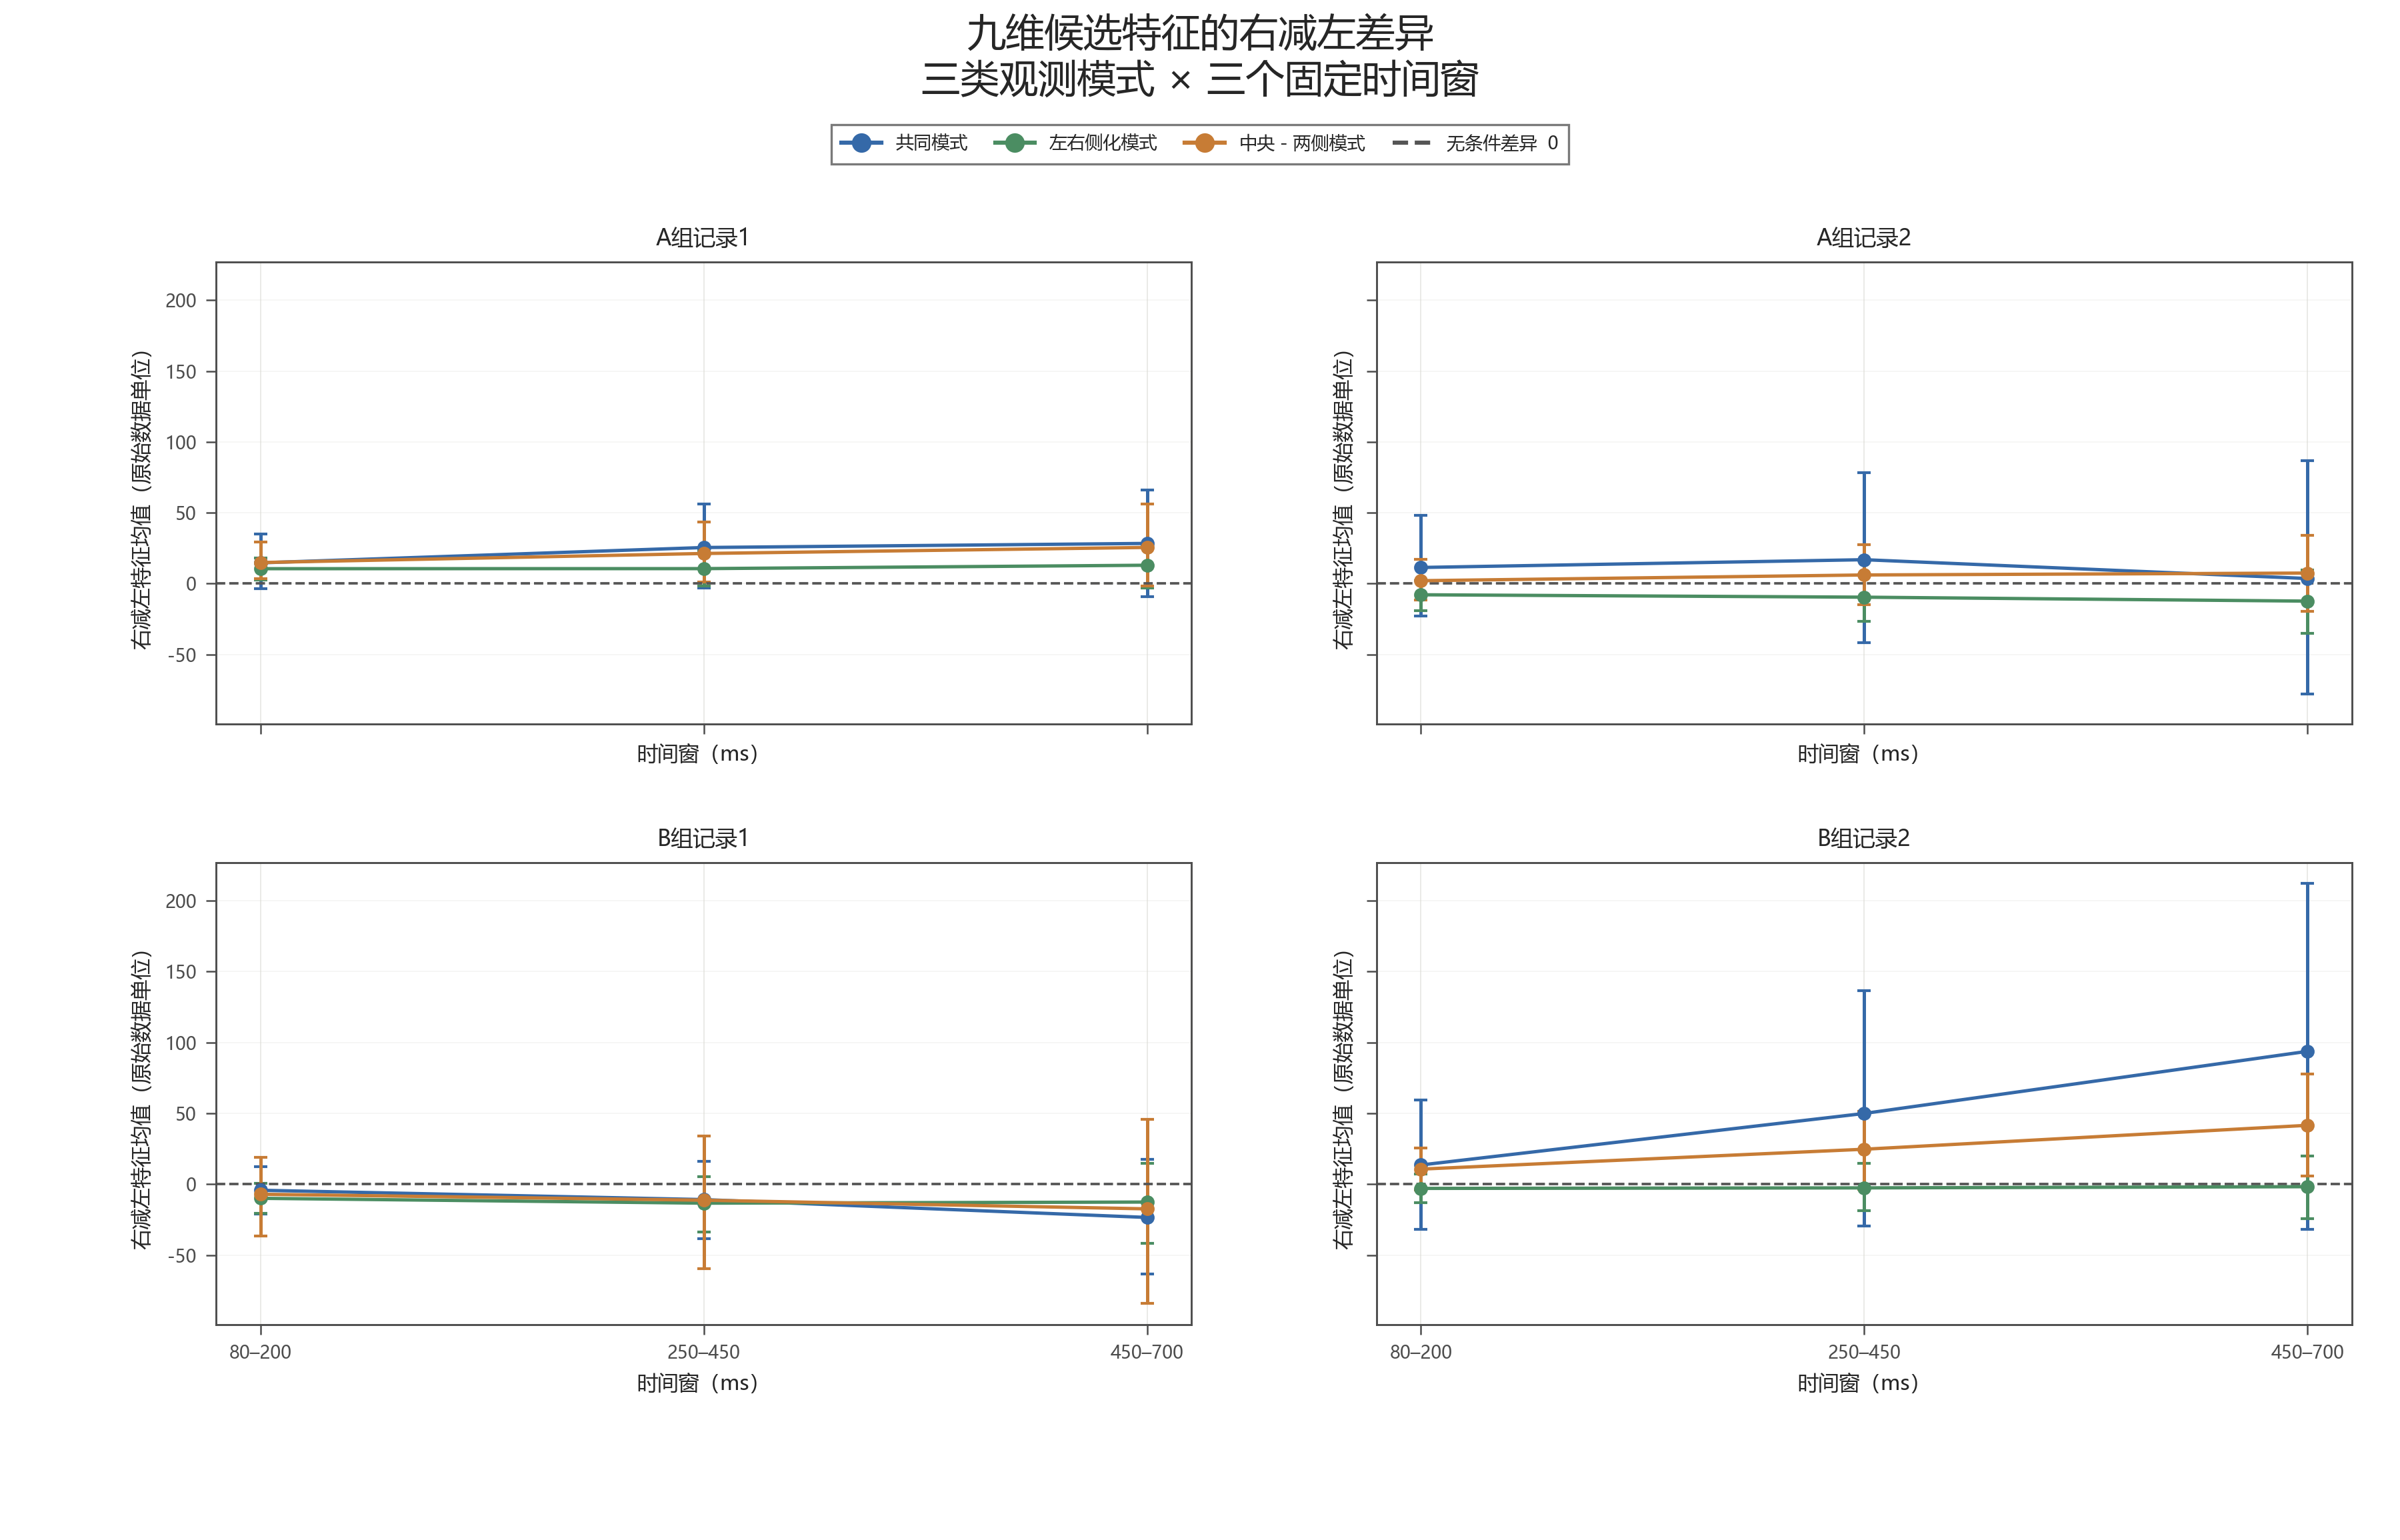
\includegraphics[width=0.94\textwidth]{src/C/q2/output/final_pic/04_九维候选特征左右差异.png}
\caption{三个观测模式的记录内右减左特征差异。横轴为辅助分析的固定时间窗，误差线为试次重采样区间；此图用于描述性比较，不是表 6 主分类特征的窗口结果。}\label{fig:q2_mode_feature_differences}
\end{figure}

分类使用收缩系数 \(0.1\) 的线性判别分析；标准化参数只由训练记录估计。该分类仅输入真实脑电，模型源变量不作为分类特征。

\subsection{结果与分析}

\subsubsection{模型内左右差异及数值核查}

在固定参数下，去除空间位置编码后模型左右差异 RMS 只保留为完整模型的 \(1.03\times10^{-5}\) 至 \(2.68\times10^{-5}\)。只保留提示 onset、去掉约 200 ms offset 后，模型差异增至完整模型的 1.22 至 1.40 倍。该对照说明当前模型内左右差异主要由空间化输入产生，提示消失阶段响应对 onset 差异有部分抵消作用。

五个源贡献经同一线性矩阵求和后重构电极预测，四折最大相对 RMS 误差为 \(2.57\times10^{-6}\)。这是实现内部的线性加和核对。模型左右差异的侧化能量比例均值为 \(0.278\)，实测为 \(0.168\)；实测各记录在 \(0.001\) 至 \(0.345\) 间变化。固定对称几何形成的模式比数据均值更侧化，未复现记录间多样的共同和形状成分。

\Needspace{8\baselineskip}
\textbf{表 3 模型内部机制核查}

\begin{longtable}{@{}p{4.0cm}p{4.6cm}p{6.2cm}@{}}
\toprule
内部核查 & 结果 & 解释范围 \\
\midrule
\endhead
去除空间位置后左右差异保留比例 & \(1.03\text{--}2.68\times10^{-5}\) & 当前模型内的空间输入依赖 \\
仅保留提示 onset 后的差异保留比例 & \(1.22\) 至 \(1.40\) & 提示 offset 活动部分抵消 onset 差异 \\
五源重构电极预测最大相对 RMS 误差 & \(2.57\times10^{-6}\) & 线性映射的数值加和核查 \\
模型/实测侧化能量比例均值 & \(0.278/0.168\) & 模型差异较实测更侧化 \\
\bottomrule
\end{longtable}

图~\ref{fig:q2_model_modes} 显示真实与模型右减左差异在三个观测模式上的比较。模型的侧化分量存在，但共同和形状分量与实测波形并未同步；源可加和只核验了代码映射关系，不意味着源代理已经由三个电极唯一识别。

\begin{figure}[H]
\centering
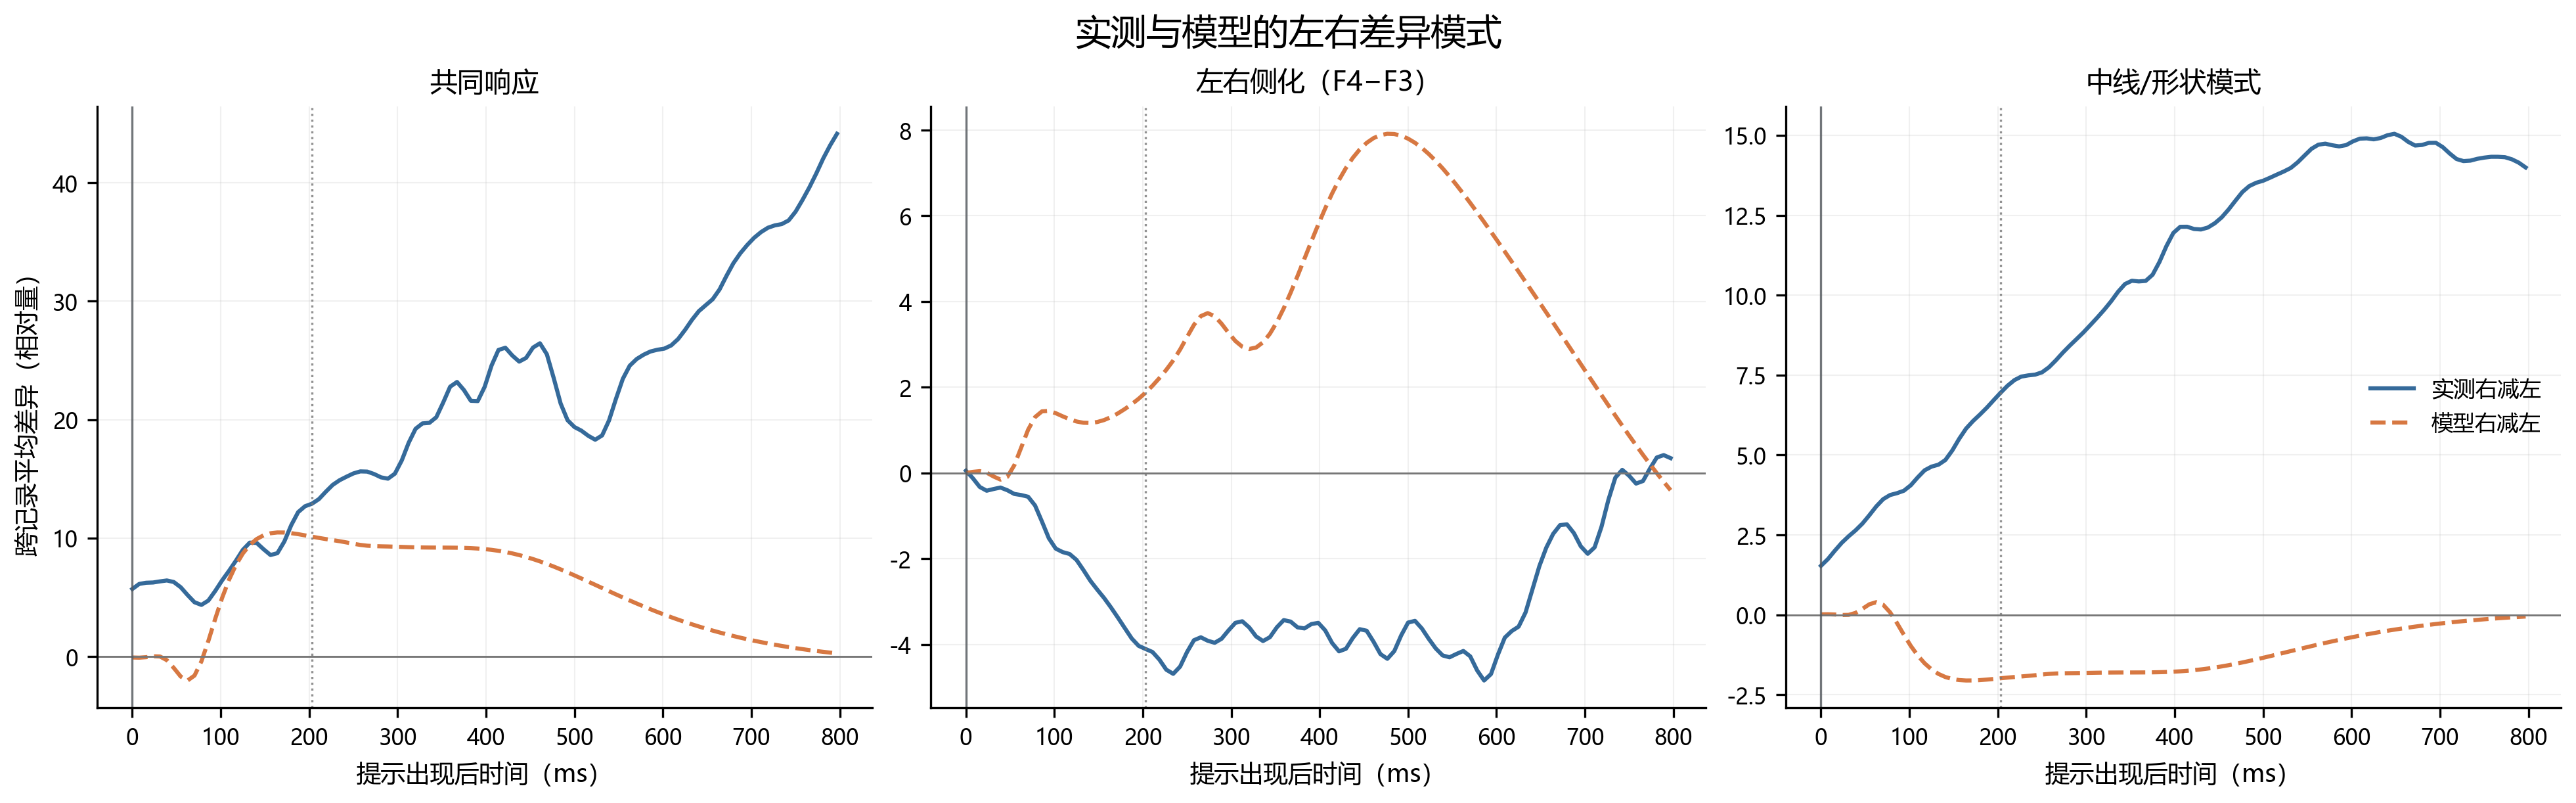
\includegraphics[width=0.96\textwidth]{src/C/q2/documents/figures/实测与模型左右差异模式.png}
\caption{实测与模型左右差异模式}\label{fig:q2_model_modes}
\end{figure}

\subsubsection{留出 ERP 拟合}

四折候选参数显示在表 4。它们描述搜索结果，优化器均未报告收敛，因此不作为已识别的生理参数。

\Needspace{12\baselineskip}

\textbf{表 4 四折候选拟合参数}

\begin{longtable}[]{@{}llllll@{}}
\toprule
留出记录 & \(\tau_s\) (ms) & \(g_i\) & \(\tau_a\) (ms) & 共享增益 \(\alpha\) & 优化状态 \\
\midrule
\endhead
A-1 & 78.87 & 0.786 & 100 & \(-63.82\) & 未收敛 \\
A-2 & 76.30 & 0.629 & 120 & \(-34.67\) & 未收敛 \\
B-1 & 76.67 & 0.909 & 120 & \(-60.36\) & 未收敛 \\
B-2 & 75.14 & 1.096 & 160 & \(-56.79\) & 未收敛 \\
\bottomrule
\end{longtable}

\textbf{表 5 留一记录留出结果}

\begin{longtable}[]{@{}llll@{}}
\toprule
留出记录 & 左右试次数 & 条件平均 NRMSE & 右减左波形相关 \\
\midrule
\endhead
A-1 & 29/25 & 4.313 & 0.098 \\
A-2 & 45/35 & 0.788 & \(-0.210\) \\
B-1 & 41/42 & 1.383 & \(-0.200\) \\
B-2 & 37/43 & 0.758 & \(-0.276\) \\
四记录总体 & 152/145 & 1.810 & \(-0.147\) \\
\bottomrule
\end{longtable}

四折拟合的 \(\tau_s\) 候选约为 75 至 79 ms，\(g_i\) 为 0.629 至 1.096，\(\tau_a\) 为 100、120、120 和 160 ms；\(\tau_a\) 仅在最后一折达到搜索上界。四折优化器均未报告收敛，且共享增益均为负值。增益的符号受源方向约定和相对尺度影响，不据此解释真实神经极性。

八个“记录 \(\times\) 左右提示”条件的平均 NRMSE 为 \(1.810\)，即误差规模大于实测 ERP 自身 RMS。右减左差异波相关均值为 \(-0.147\)，说明模型预测的差异波与实测差异波在形状上未呈现正相关；当前参数下模型未复现观测到的左右差异波形。A-2 和 B-2 的条件平均 NRMSE 低于 1，但 A-1 为 4.313，B-1 为 1.383；总体结果不支持当前模型已稳定复现真实 ERP。图~\ref{fig:q2_heldout_erp} 给出各记录和电极的完整留出曲线。

\begin{figure}[H]
\centering
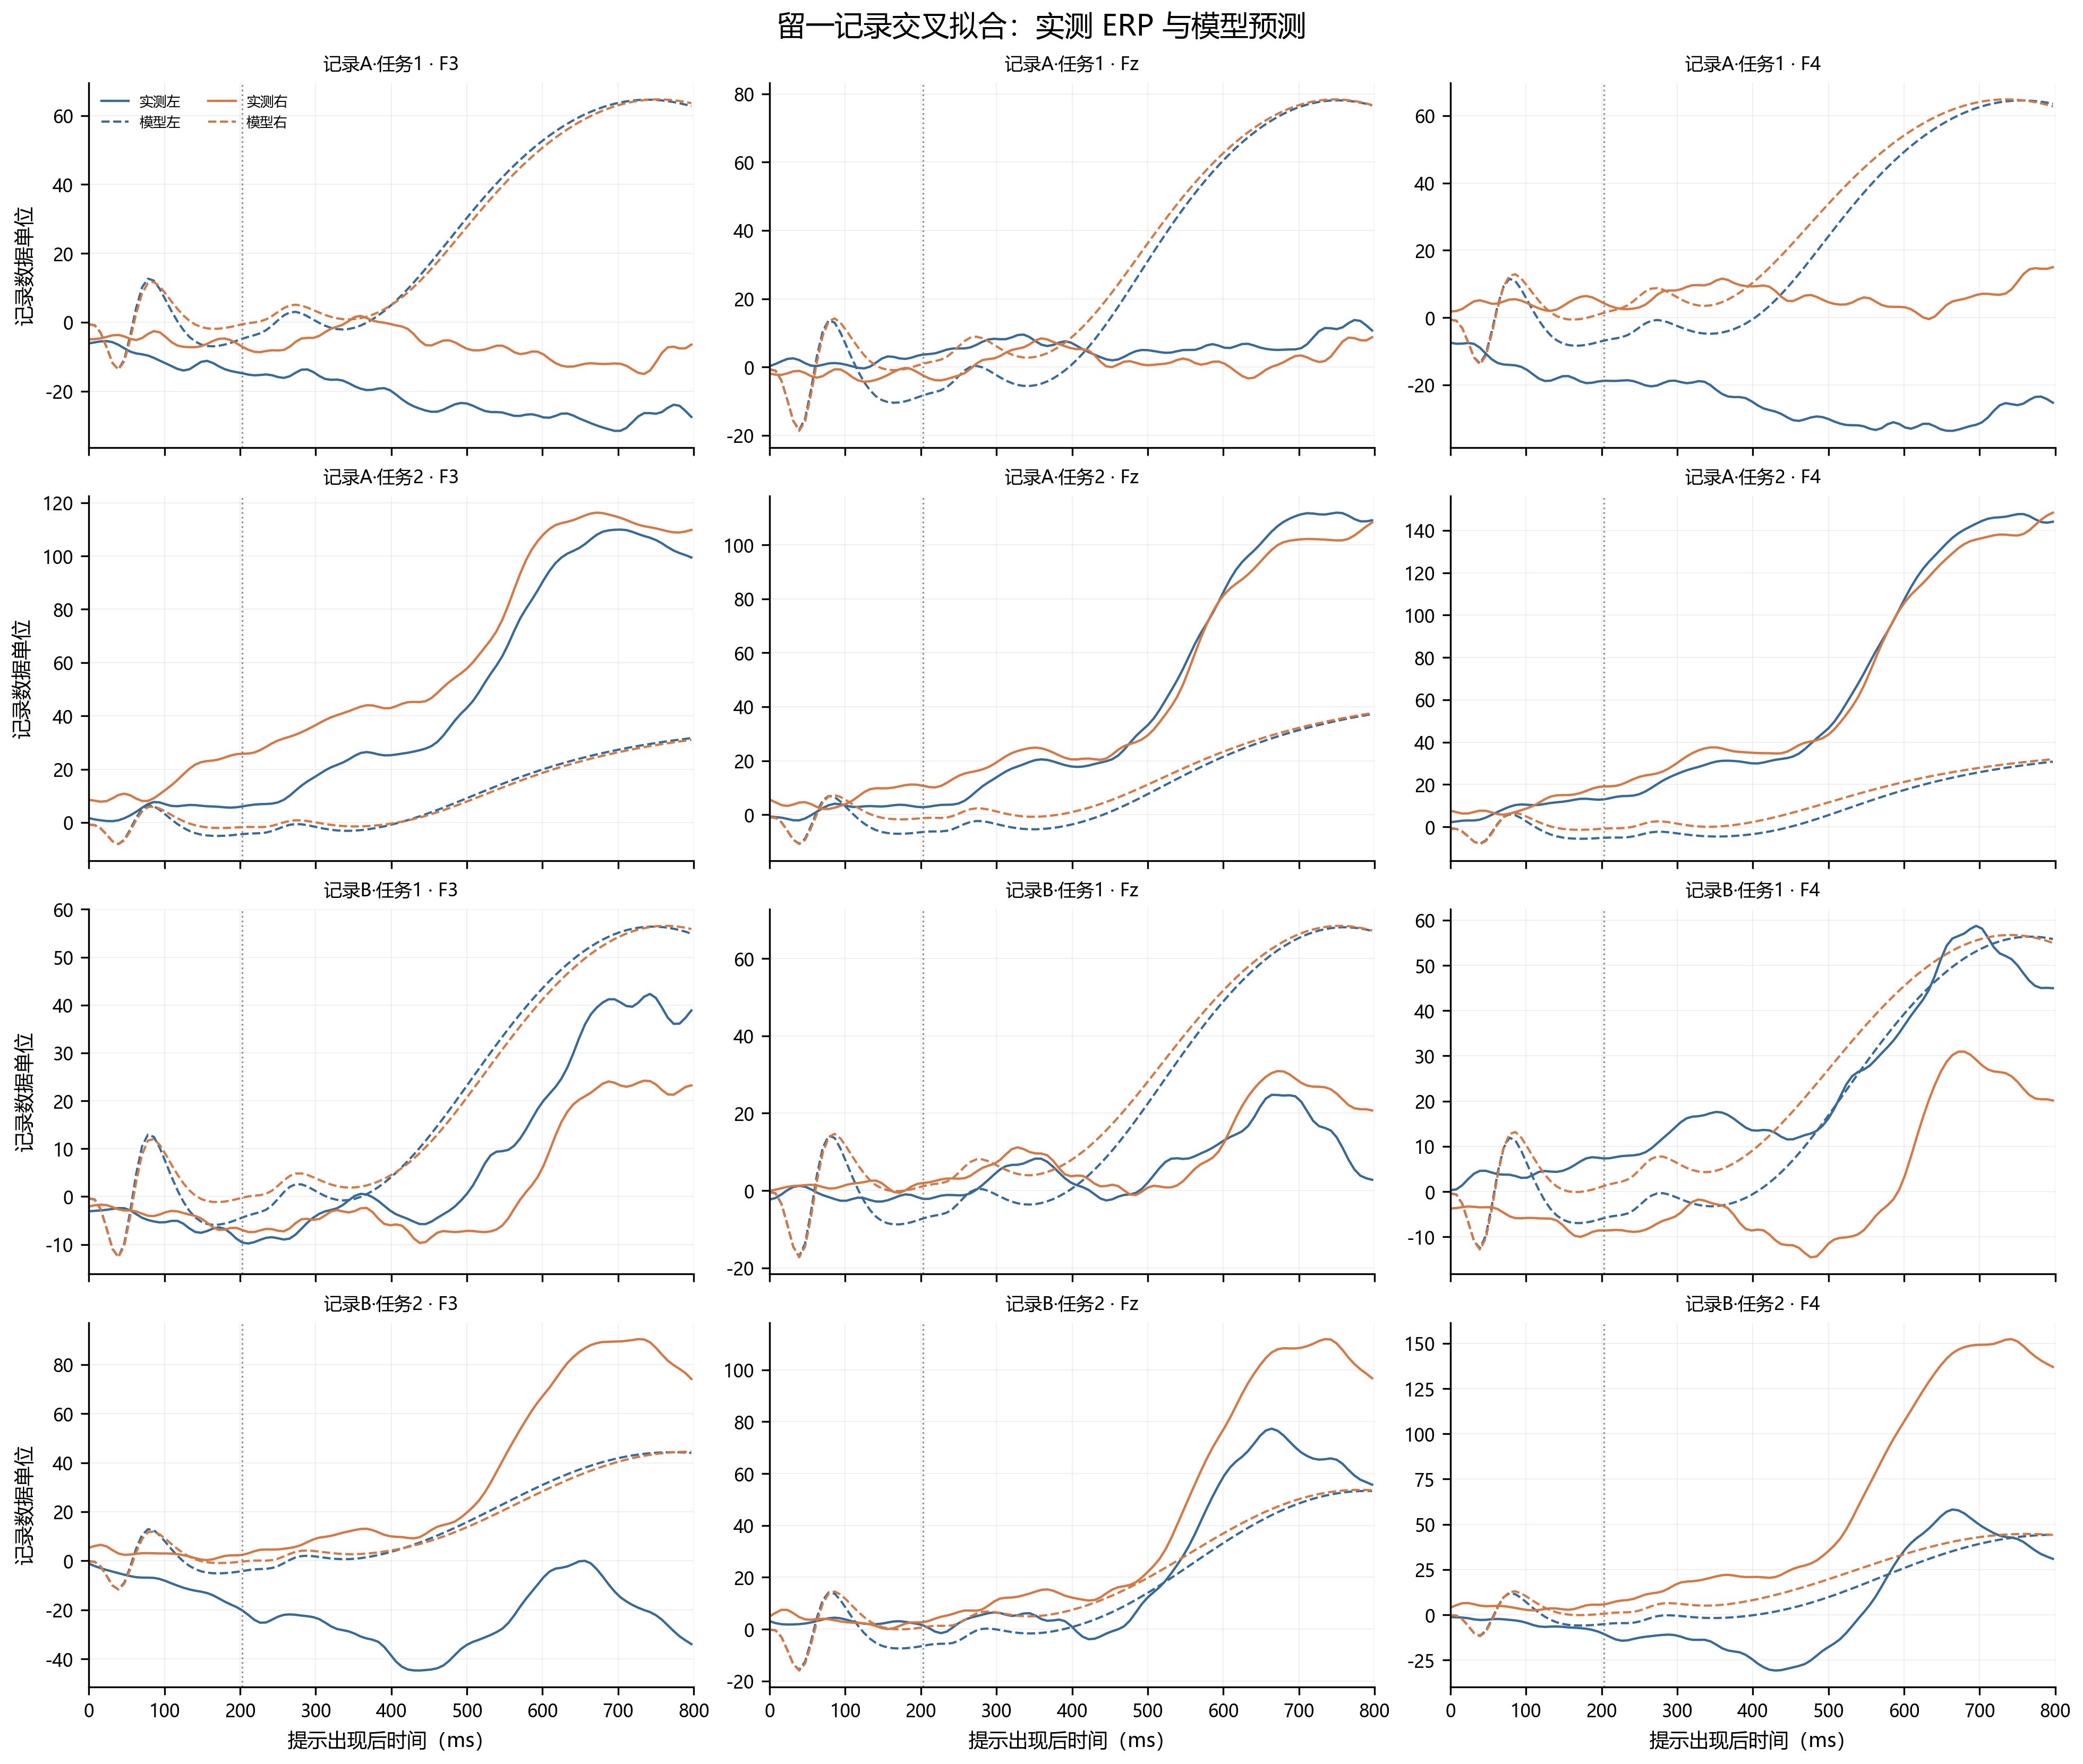
\includegraphics[width=0.96\textwidth]{src/C/q2/documents/figures/留一记录实测与模型ERP.png}
\caption{留一记录实测 ERP 与模型预测}\label{fig:q2_heldout_erp}
\end{figure}

\Needspace{12\baselineskip}

\subsubsection{九维脑电特征及分类结果}

\textbf{表 6 九维固定特征的留一记录分类}

\begin{longtable}[]{@{}llll@{}}
\toprule
留出记录 & 试次数 & 平衡准确率 & AUC \\
\midrule
\endhead
A-1 & 54 & 0.347 & 0.309 \\
A-2 & 80 & 0.494 & 0.488 \\
B-1 & 83 & 0.517 & 0.517 \\
B-2 & 80 & 0.504 & 0.490 \\
记录宏平均 & 297 & 0.466 & 0.451 \\
\bottomrule
\end{longtable}

九维特征宏平均平衡准确率为 \(46.6\%\)，宏平均 AUC 为 \(0.451\)，两个指标均未超过 \(0.5\)。四个外层记录中，只有两个平衡准确率略高于 \(0.5\)，单个高于机会水平的记录不足以构成跨记录结论。九维向量给出了一个可计算、可复核的传感器表征，但当前运行没有验证其能稳定区分左右提示；该结论也不能反推左右脑电差异不存在。

图~\ref{fig:q2_heldout_class} 逐折显示该特征的平衡准确率与 \(50\%\) 参考线。记录间差异和低宏平均值说明现有特征及数据条件下的跨记录泛化有限。

\begin{figure}[H]
\centering
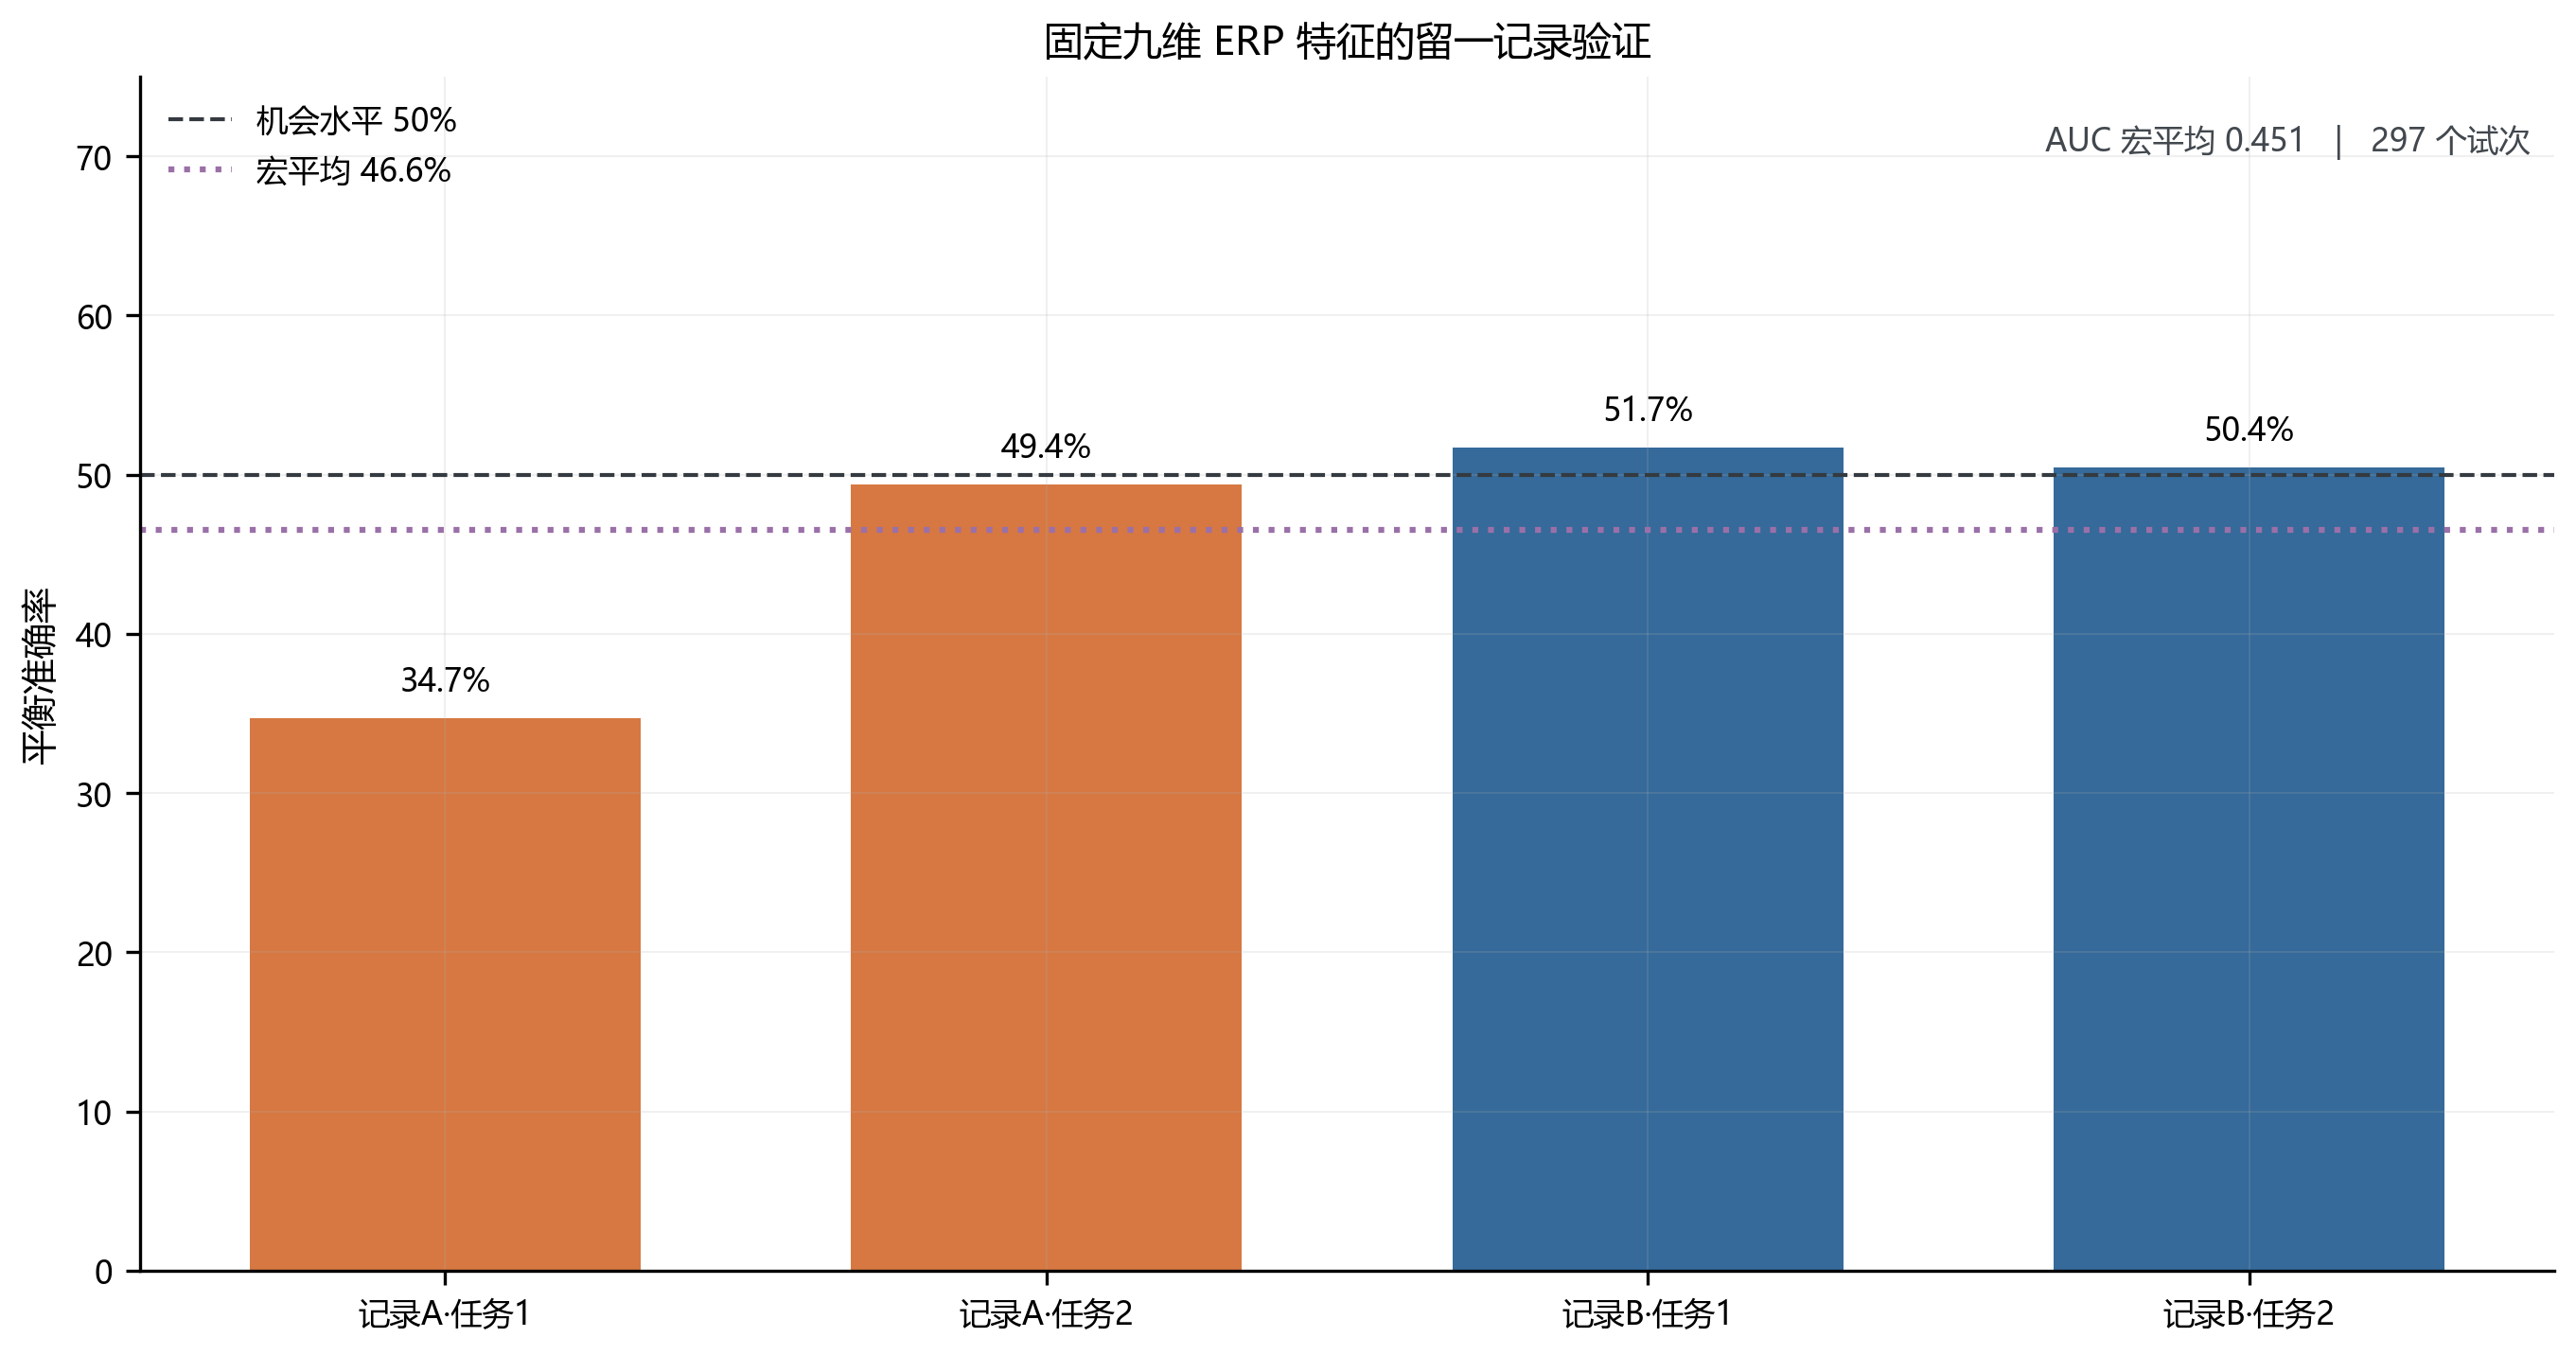
\includegraphics[width=0.96\textwidth]{src/C/q2/documents/figures/九维ERP特征_留一记录分类.png}
\caption{九维 ERP 特征留一记录分类}\label{fig:q2_heldout_class}
\end{figure}

\subsubsection{记录内随机五折的补充结果}

为展示与留一记录验证不同的记录内表现，图~\ref{fig:q2_random_cv} 和图~\ref{fig:q2_random_scores} 给出按记录分层的随机五折折外预测。该图对应随机划分探索中命中的第 3 轮（种子 20260928）：记录宏平均平衡准确率和合并试次准确率均为 55.6\%。同一记录的试次同时进入训练折与测试折，且展示轮次经过多轮随机搜索筛选；因此，该结果可能受记录内共享结构和轮次选择影响，只作为补充的探索性描述，不作为泛化性能估计。本文主分类结论仍以整份记录留出的 46.6\% 宏平均平衡准确率和 0.451 AUC 为准。

\begin{figure}[H]
\centering
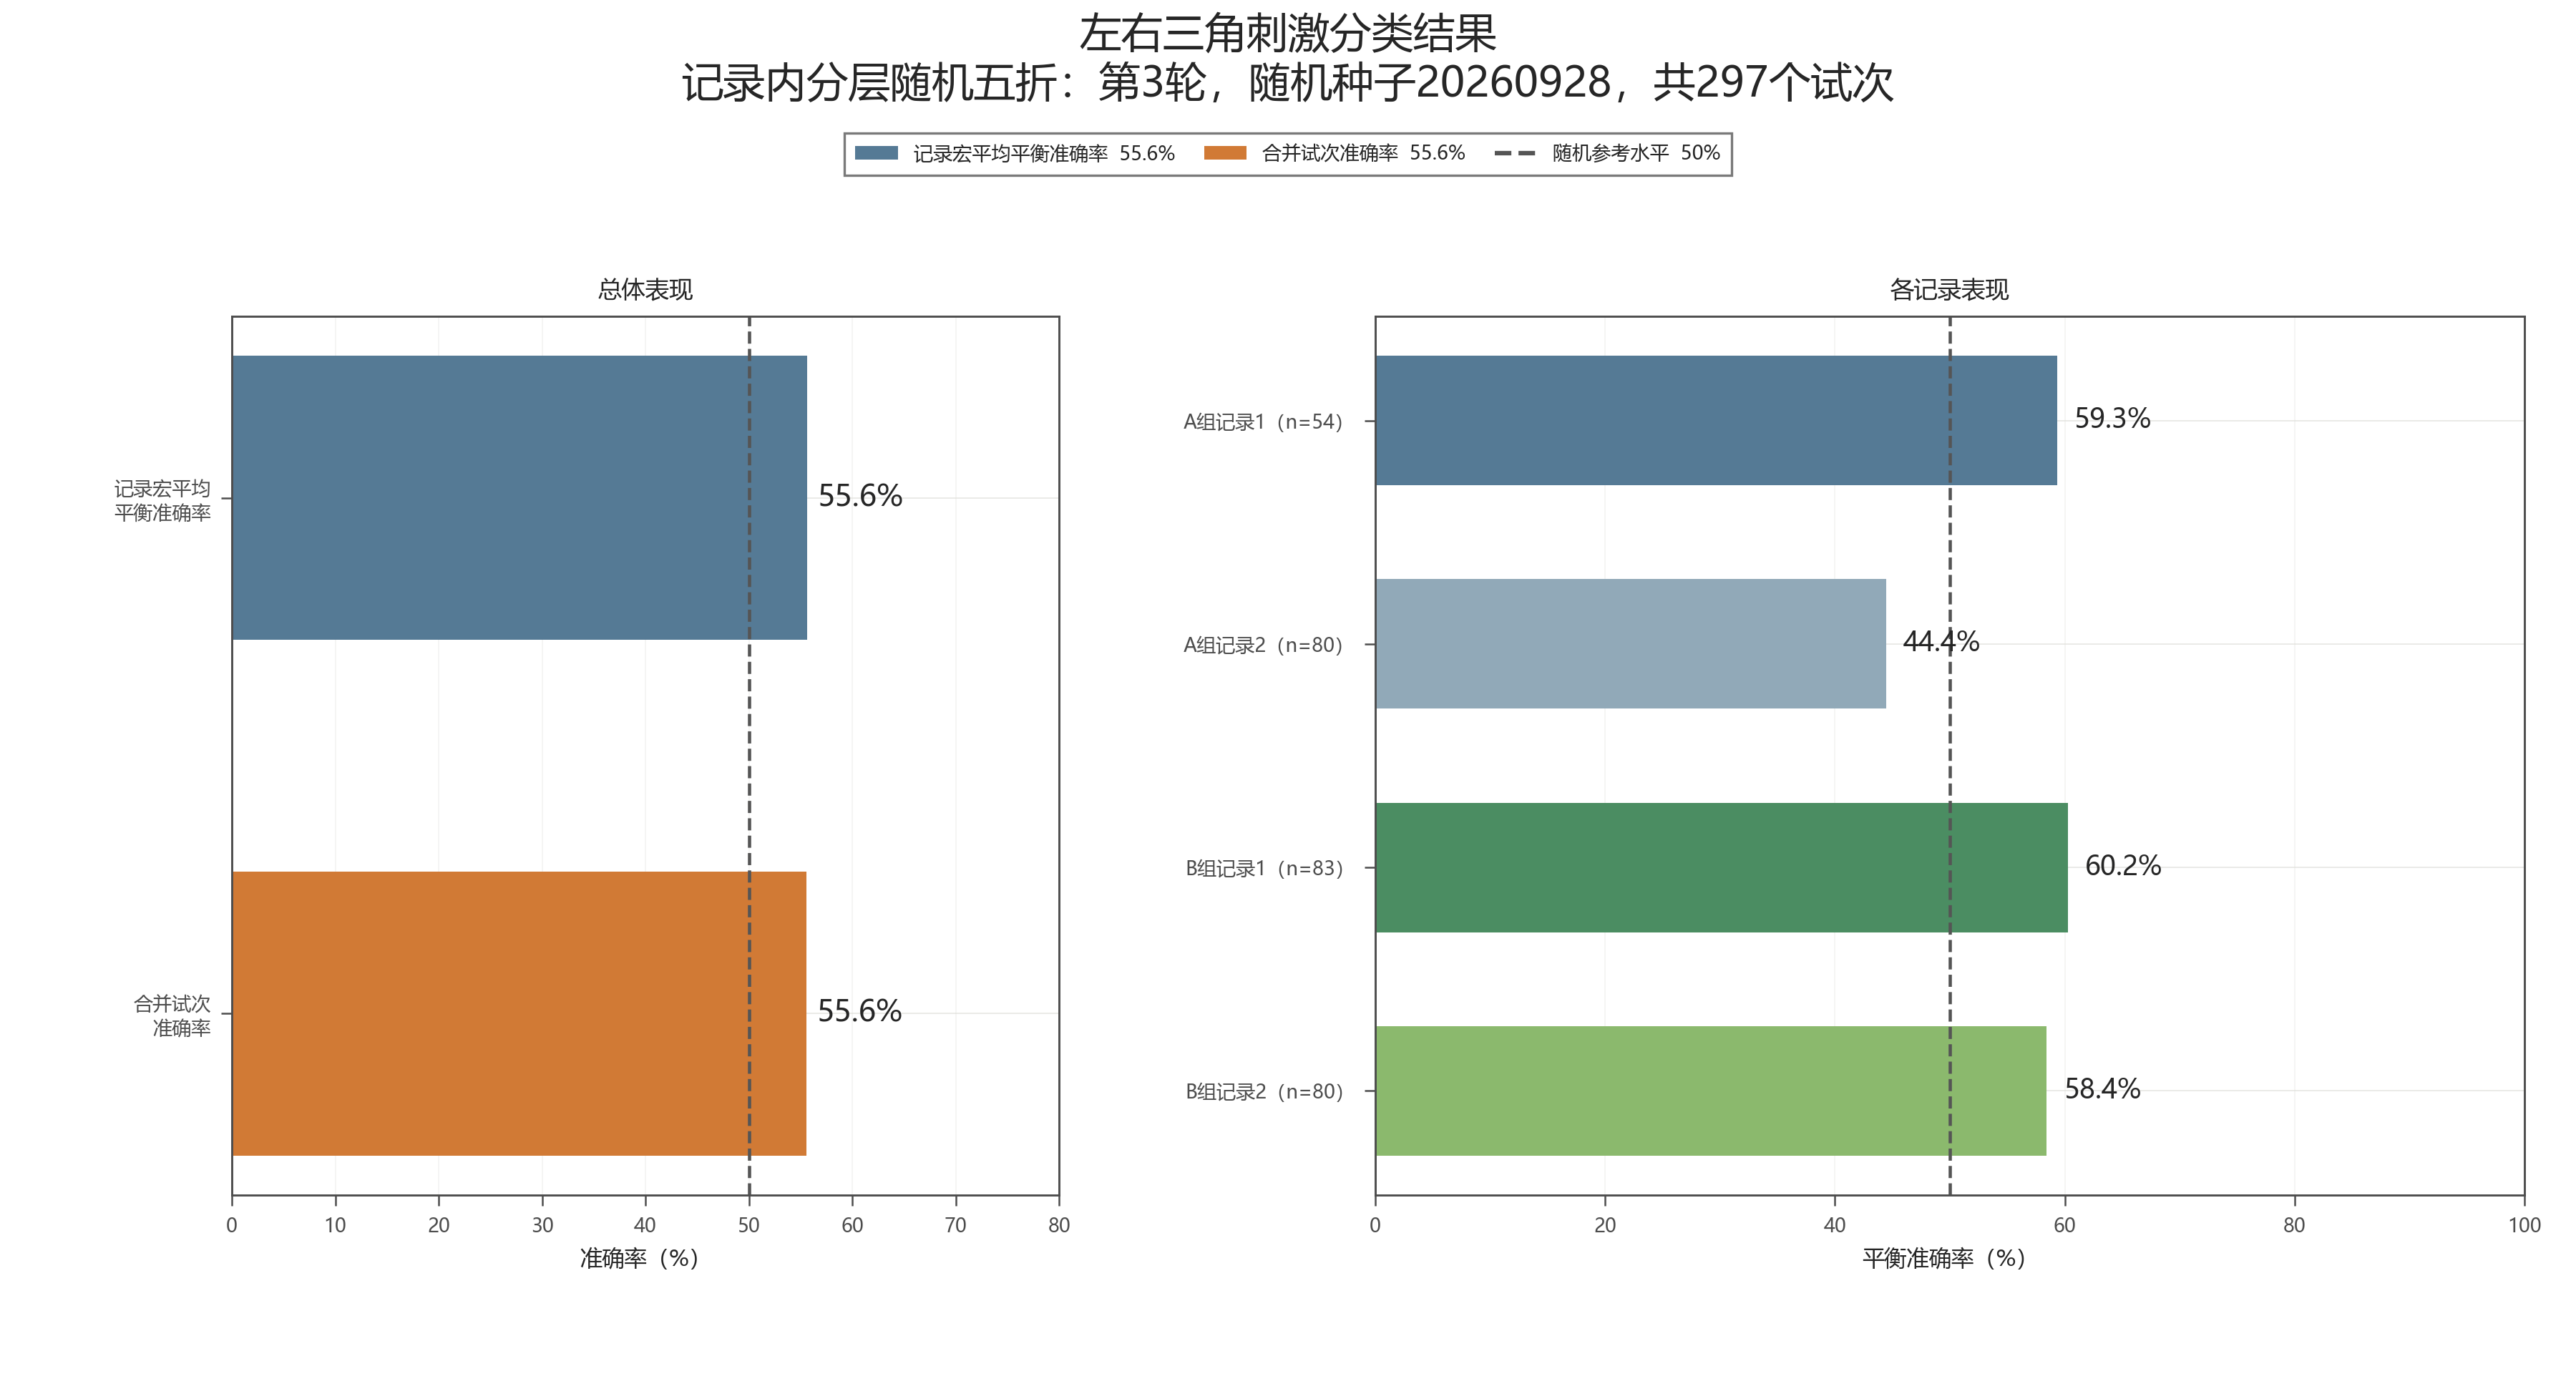
\includegraphics[width=0.94\textwidth]{src/C/q2/output/final_pic/01_随机五折分类结果.png}
\caption{记录内分层随机五折的辅助分类结果。图中记录宏平均平衡准确率与合并试次准确率均为 55.6\%；该随机搜索命中轮次不替代整份记录留出验证。}\label{fig:q2_random_cv}
\end{figure}

\begin{figure}[H]
\centering
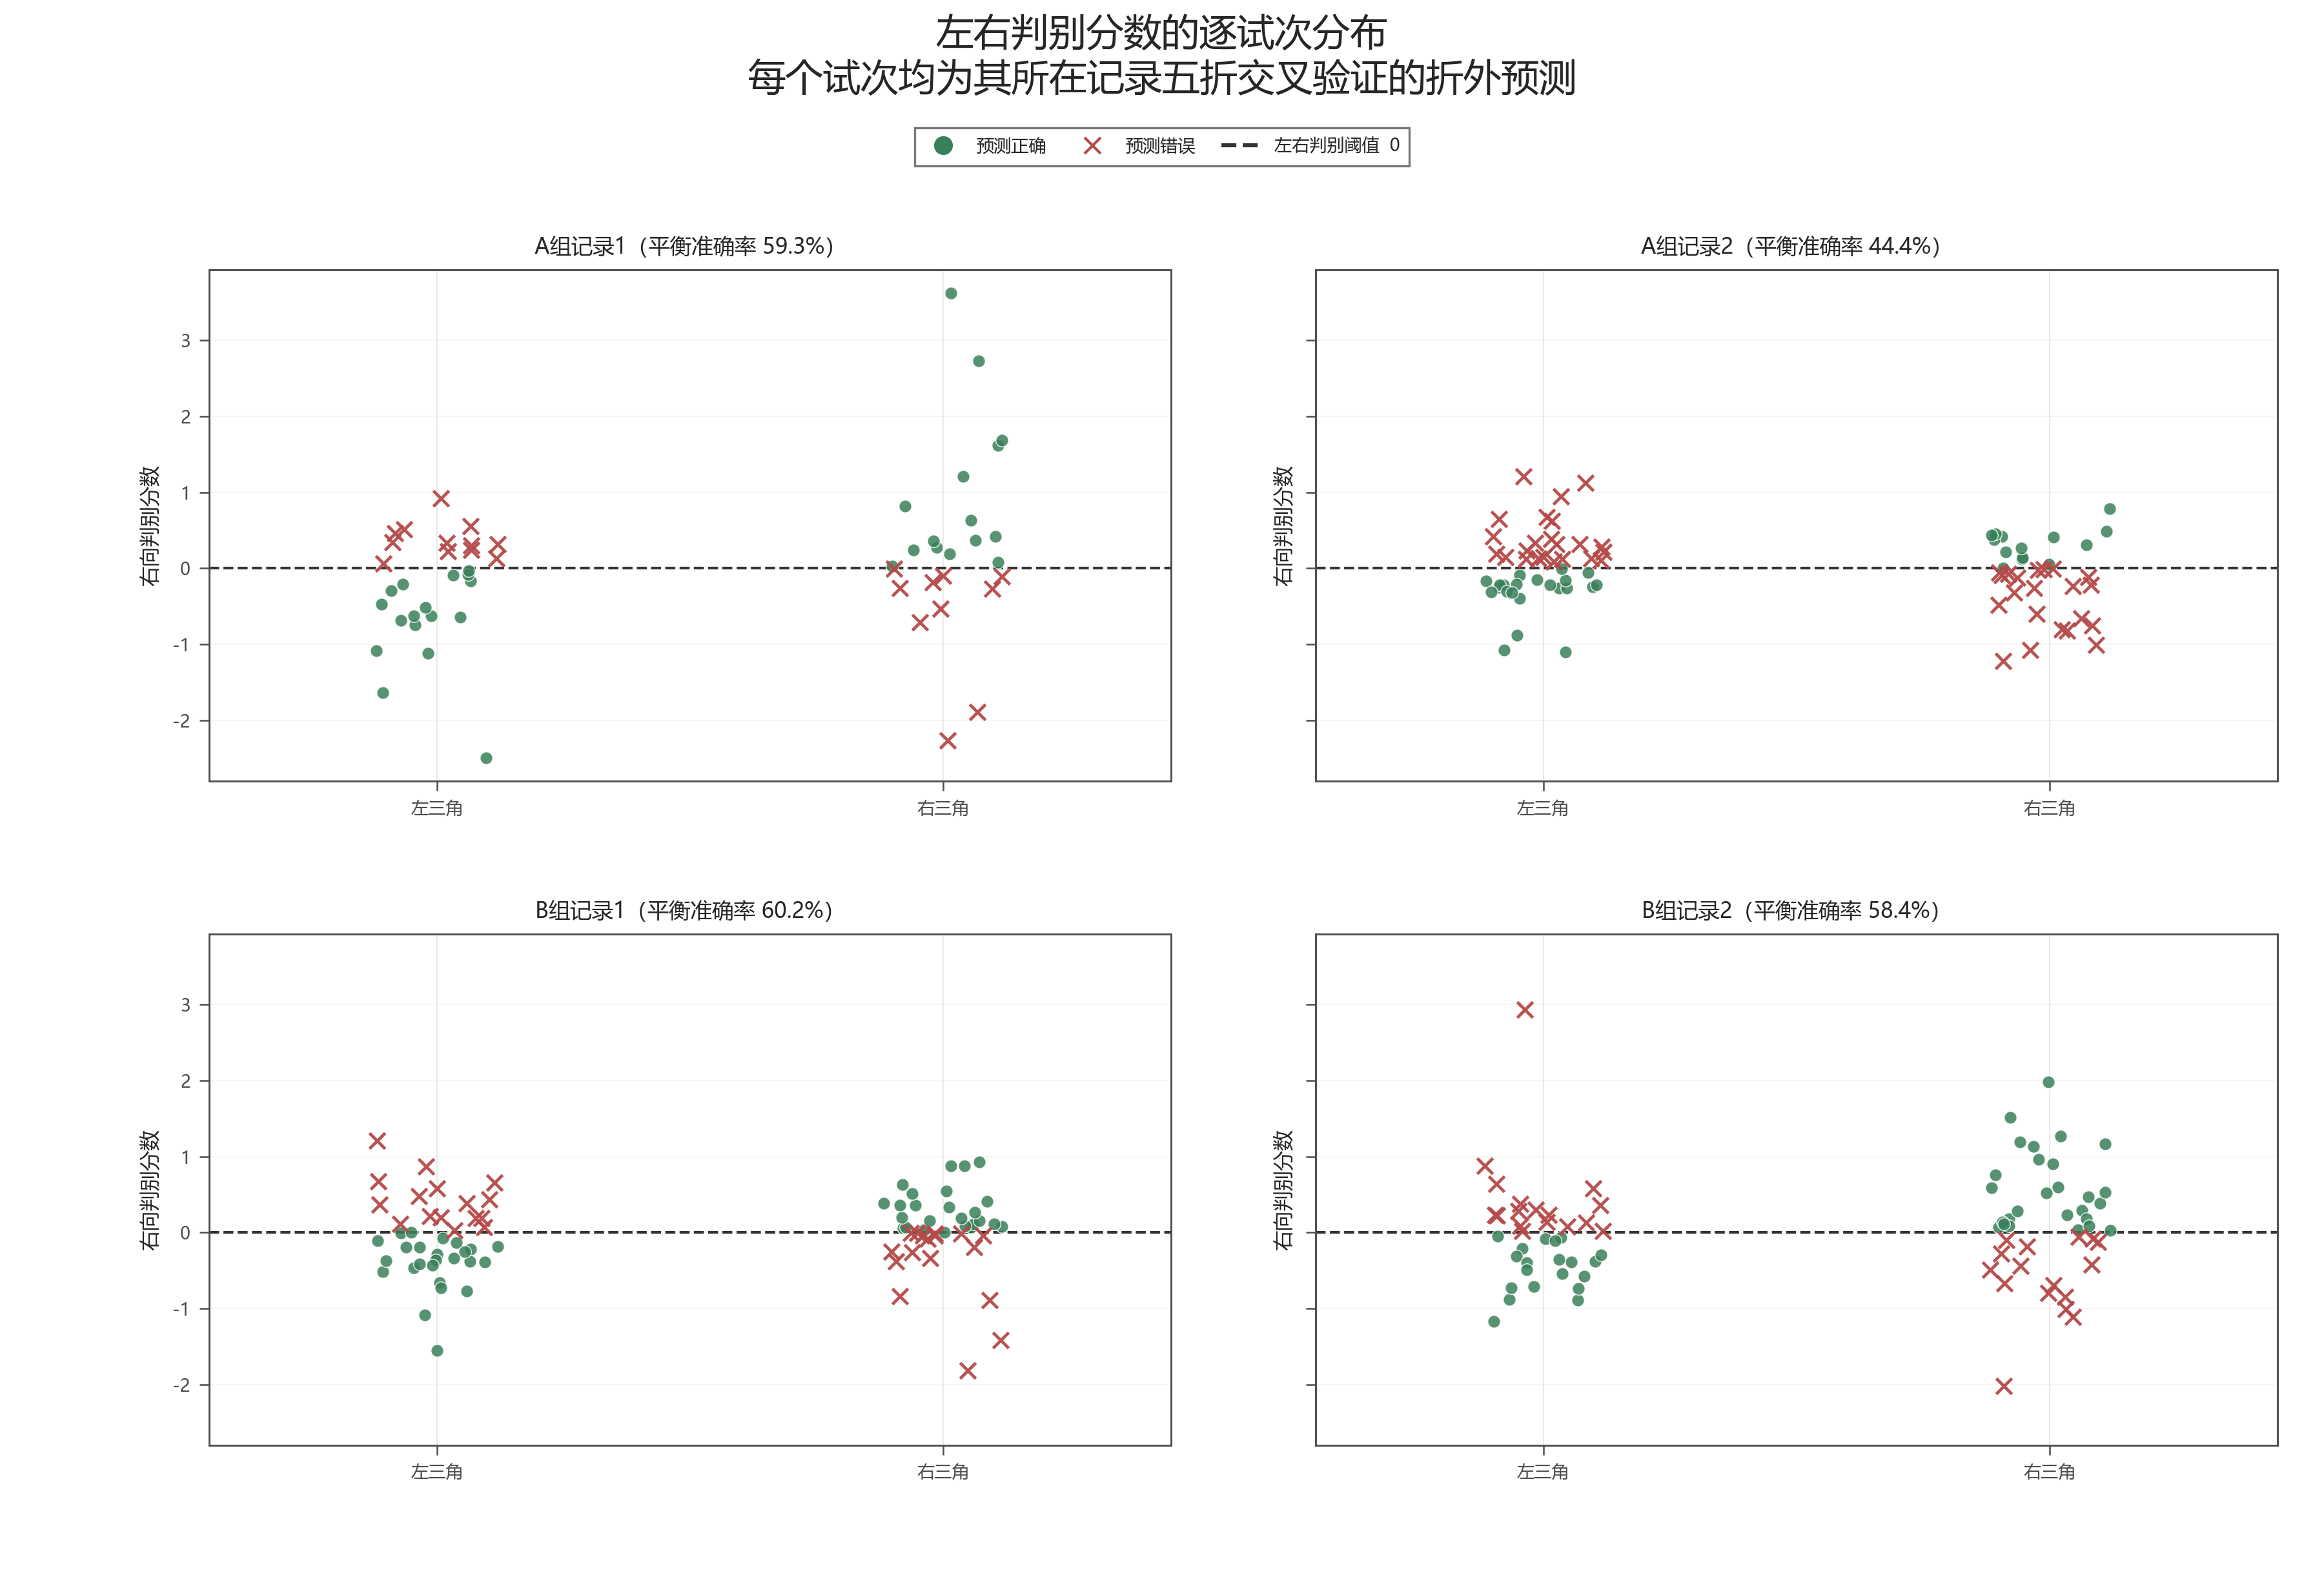
\includegraphics[width=0.94\textwidth]{src/C/q2/output/final_pic/02_逐试次判别分数.png}
\caption{记录内随机五折的逐试次折外判别分数。圆点为正确预测，叉号为错误预测，虚线为左右判别阈值；分数分布仅反映该探索轮次。}\label{fig:q2_random_scores}
\end{figure}

\subsection{本章小结}

本模型的计算路径从视觉像素出发，经明暗适应、方向和构型特征、兴奋-抑制动力学及固定头皮正向映射到三个电极；左右差异可以逐级追踪。拟合和分类使用不同的数据单位与目的：平均 ERP 留出检验波形生成能力，单试次九维特征检验方向标签的跨记录可分性。留出拆分按整份 MAT 记录进行，降低了同一记录同时参与拟合和评价造成的信息共享。

针对题目要求的三个目标，本模型的回应如下。第一，关于“从 LGN 到皮层再到头皮的机理”，模型给出了从视觉亮度差分、LGN ON/OFF 适应中继、Gabor 方向与三角构型编码、三组兴奋-抑制群体，到五源代理和固定头皮正向映射的完整计算路径，每一步都可逐级复核。第二，关于“左右三角刺激差异的形成机制”，模型内部消融显示左右差异主要由空间位置编码产生；去除空间位置后差异 RMS 仅保留为完整模型的 \(10^{-5}\) 量级，提示消失阶段响应对 onset 差异有部分抵消。第三，关于“可区分两类视觉刺激响应的特征表示”，本文提出了一个直接由真实单试次 EEG 计算的九维固定特征，并给出可复核的留出分类基线；该特征在当前四份记录上未表现出稳定的跨记录区分能力，但作为可计算基线可供后续记录进一步检验。

结论仍受四项限制。第一，四份记录没有独立受试者标识，结果不构成跨个体验证。第二，模型只生成提示响应，未生成约 2.2 s 目标事件；零相位滤波会使完整试次的后续活动影响较早时刻，绝对 ERP 误差因此依赖事件上下文。第三，均匀无限导体点偶极映射和规范源坐标没有个体 MRI、真实参考配置及源电流标定，源代理和头皮输出不具备解剖或微伏解释。第四，外层优化均未收敛且分类指标低于机会水平；因此参数、机制及特征应作为当前数据下的待验证模型，而非已确立的生理规律或稳定解码器。
